\documentclass{statsmsc}

\title{Extending Sparse Bayesian Model Identification to Polynomial Models with Errors-in-Variables Regression}
\author{Xinyi Zhang}
\CID{06006350}
\supervisor{Guy Nason and Lloyd Fung}
\date{1 August 2025}
%For today's date, use:
%\date{\today}
\logoimg{}

% THIS IS WHERE NEW COMMANDS CAN BE DEFINED

% commands below only used in the proof; otherwise can be deleted
\newcommand{\consta}{a}
\newcommand{\X}{X}
\newcommand{\EE}[1]{ \mathrm{E} [ #1 ] }
\newcommand{\inparenth}[1]{\left( #1 \right)}

\usepackage{xcolor}
\usepackage{hyperref}
\usepackage{amsmath}
\usepackage{booktabs}
\hypersetup{
    colorlinks,
    linkcolor={blue!50!black},
    citecolor={blue!50!black},
    urlcolor={blue!50!black}
}


\begin{document}

% Generates the Title Page
\maketitle

% Generates plagiarism declaration
\declarationname{Xinyi Zhang}
\declarationdate{20 August 2025}
\declaration 

\begin{acknowledgements}
    I would like to express my sincere gratitude to my supervisors, Professor Guy Nason and Dr. Lloyd Fung, for their invaluable guidance and constructive feedback throughout the development of this thesis. I am especially grateful to Dr. Fung for his encouragement and continuous support during the course of my research, which has been instrumental in helping me complete this work.
\end{acknowledgements}

%=================================================================
% VERY IMPORTANT
% This command switches from Roman to Arabic numbering for main part of report. Do not modify.
\mainmatter
%=================================================================


\begin{abstract}
    Direct discovery of governing equations remains a central challenge in scientific machine learning, especially under noisy measurement conditions. This thesis develops two frameworks for sparse polynomial model selection. First, we introduce a Bayesian evidence–based approach that directly computes posterior model probabilities, thereby implementing Occam’s razor in a principled way. This framework addresses the case where noise is present only in the response variable, balancing model fit with parsimony without relying on asymptotic approximations such as Akaike Information Criterion (AIC) or Bayesian Information Criterion (BIC). Second, to tackle the more challenging error-in-variables (EIV) problem where both predictors and responses are noisy, we propose the Sequentially Thresholded Least Squares with Orthogonal Distance Regression (STLSQ-ODR). This method combines sparse identification of nonlinear dynamics (SINDy) with ODR’s ability to correct for measurement error, providing robust recovery of governing equations under Gaussian, heavy-tailed, or correlated noise. 
    Simulation studies demonstrate that the Bayesian razor effectively identifies parsimonious models when noise is confined to the response variable, while STLSQ-ODR provides more reliable recovery under the EIV problem. 
    Across noise structures, BIC-based thresholding consistently outperforms OLS-based selection in stability, although all methods deteriorate under extreme noise. Overall, the findings highlight Bayesian evidence and ODR regression as complementary approaches for sparse model discovery under noisy conditions, laying the groundwork for extensions to higher-dimensional and practical applications.
\end{abstract}

%===============================================================
%
% Students please remove the General tips when submitting your report
%
%===============================================================


\section{Introduction}
\label{sec:intro}

Direct equation discovery continues to represent a key challenge and area of progress in scientific machine learning.
From a model selection perspective, it is important to guard against overfitting, since this compromises its ability to generalise and provide reliable forecasts. At the same time, we also want to enhance the interpretability and parsimony of the model. Thus, it is crucial to balance accuracy with interpretability and parsimony. These principles align with Occam’s razor, which states that among competing hypotheses that explain the data, the simplest one consistent with the observations should be preferred. 
The motivation is twofold: aesthetically, mathematically elegant theories are often considered more likely to be correct; empirically, simpler models tend to make more precise predictions, whereas complex models require more assumptions and are prone to overfitting (see \cite{mackay2003}). The Bayesian evidence and sparse identification of nonlinear dynamics (SINDy) are regarded as principled methods for model selection across statistics, machine learning, and the natural sciences because they naturally embody the principle of Occam’s razor.


Bayesian evidence provides a principled framework for implementing Occam's razor, with its theoretical foundation laid by David MacKay and Stephen Gull.
\cite{mackay1992} showed that the evidence integral $Z = \int P(\text{data} \mid \theta)\, P(\theta)\, \mathrm{d}\theta$
can be decomposed into a likelihood term measuring goodness-of-fit and an Occam factor that penalises unnecessary model complexity. This penalty enforces parsimony by down-weighting parameter dimensions that are not effectively constrained by the data, thereby discouraging overfitting. 
In parallel, \cite{gull1988} provided an information-theoretic justification for prior specification via the Maximum Entropy Principle, emphasising how the choice of prior encodes assumptions about model simplicity. This perspective later motivated the use of sparsity-inducing priors, such as the Laplace distribution \citep{park2008} and spike-and-slab formulations \citep{mitchell1988, george1993}, which concentrate probability mass near zero and thereby favour models where only a small subset of parameters are active.
The practical computation of Bayesian evidence has stimulated the development of specialised numerical methods. Nested Sampling \citep{buchner2016,buchner2023} and Thermodynamic Integration (TI) \citep{aponte2022} are among the most widely used algorithms for evaluating the evidence integral, with the former based on stochastic exploration of constrained likelihood contours and the latter grounded in statistical physics and particularly popular in cognitive and neurodynamical modelling. The Laplace approximation \citep{mackay2003} provides a computationally efficient alternative by performing a local quadratic expansion around the maximum a posteriori (MAP) estimate, though at the cost of reduced accuracy when the posterior is highly non-Gaussian. 
Building on these theoretical and computational advances, a large body of work (see, e.g., \cite{rougier2021, bayarri2012}) demonstrates that the marginal likelihood, or evidence, automatically balances data fit with model complexity, thereby embodying Occam’s razor without the need for ad-hoc penalisation. More recent contributions \citep{lotfi2022, knuth2015} further highlight both the strengths and limitations of evidence-based model comparison, particularly in high-dimensional and data-scarce regimes. Together, these studies establish Bayesian evidence as not only a theoretical embodiment of Occam’s razor but also a practical criterion for selecting parsimonious models that generalise well.


SINDy’s Sequentially Thresholded Least Squares (STLSQ) algorithm provides another useful framework for addressing the issue of overfitting in model selection. SINDy essentially reformulates equation discovery into a sparse dictionary learning framework, which can be used for model selection. 
It first generates a library containing all possible candidate functions of the data, and subsequently employs sparse regression to identify the functions that meaningfully represent the underlying dynamics, filtering out the superfluous ones. By enforcing parsimony through sparsity, SINDy yields interpretable models that strike a balance between accuracy and generalizability, while its streamlined structure also enables comparatively efficient and rapid learning relative to many other machine learning approaches.
SINDy has progressed markedly in recent years. Researchers have proposed a series of new algorithms, such as uncertainty quantification SINDy (UQ-SINDy), developed by \cite{hirsh2022}. They used MCMC and sparsifying priors; Ensemble-SINDy (E-SINDy), proposed by \cite{fasel2022}, which used the idea of bootstrap aggregating; and a rapid Bayesian identification framework constructed by \cite{fung2024} to address problems with scarce and noisy data. 


However, in computing the likelihood and posterior distribution, the current method is challenged by how uncertainty exists in both the dependent and independent variables. Since the principle of SINDy is to regress the derivatives of the time series against the time series itself, when there is uncertainty in the time series, it propagates through both the dependent and independent variables in the regression process. This setting, in which measurement noise affects both the predictors and the response, is known as the errors-in-variables (EIV) problem. 
However, despite the growing maturity of Bayesian SINDy methods, they are almost all built upon a common, standard regression assumption: that the model primarily accounts for noise in the dependent variable (the time derivative $\dot{x} $), while ignoring the fact that the state variables $x$, which serve as the independent variables, are themselves inevitably derived from noisy measurements. This violates a fundamental premise of regression analysis and may lead to systematic bias in model selection.


\begin{figure}
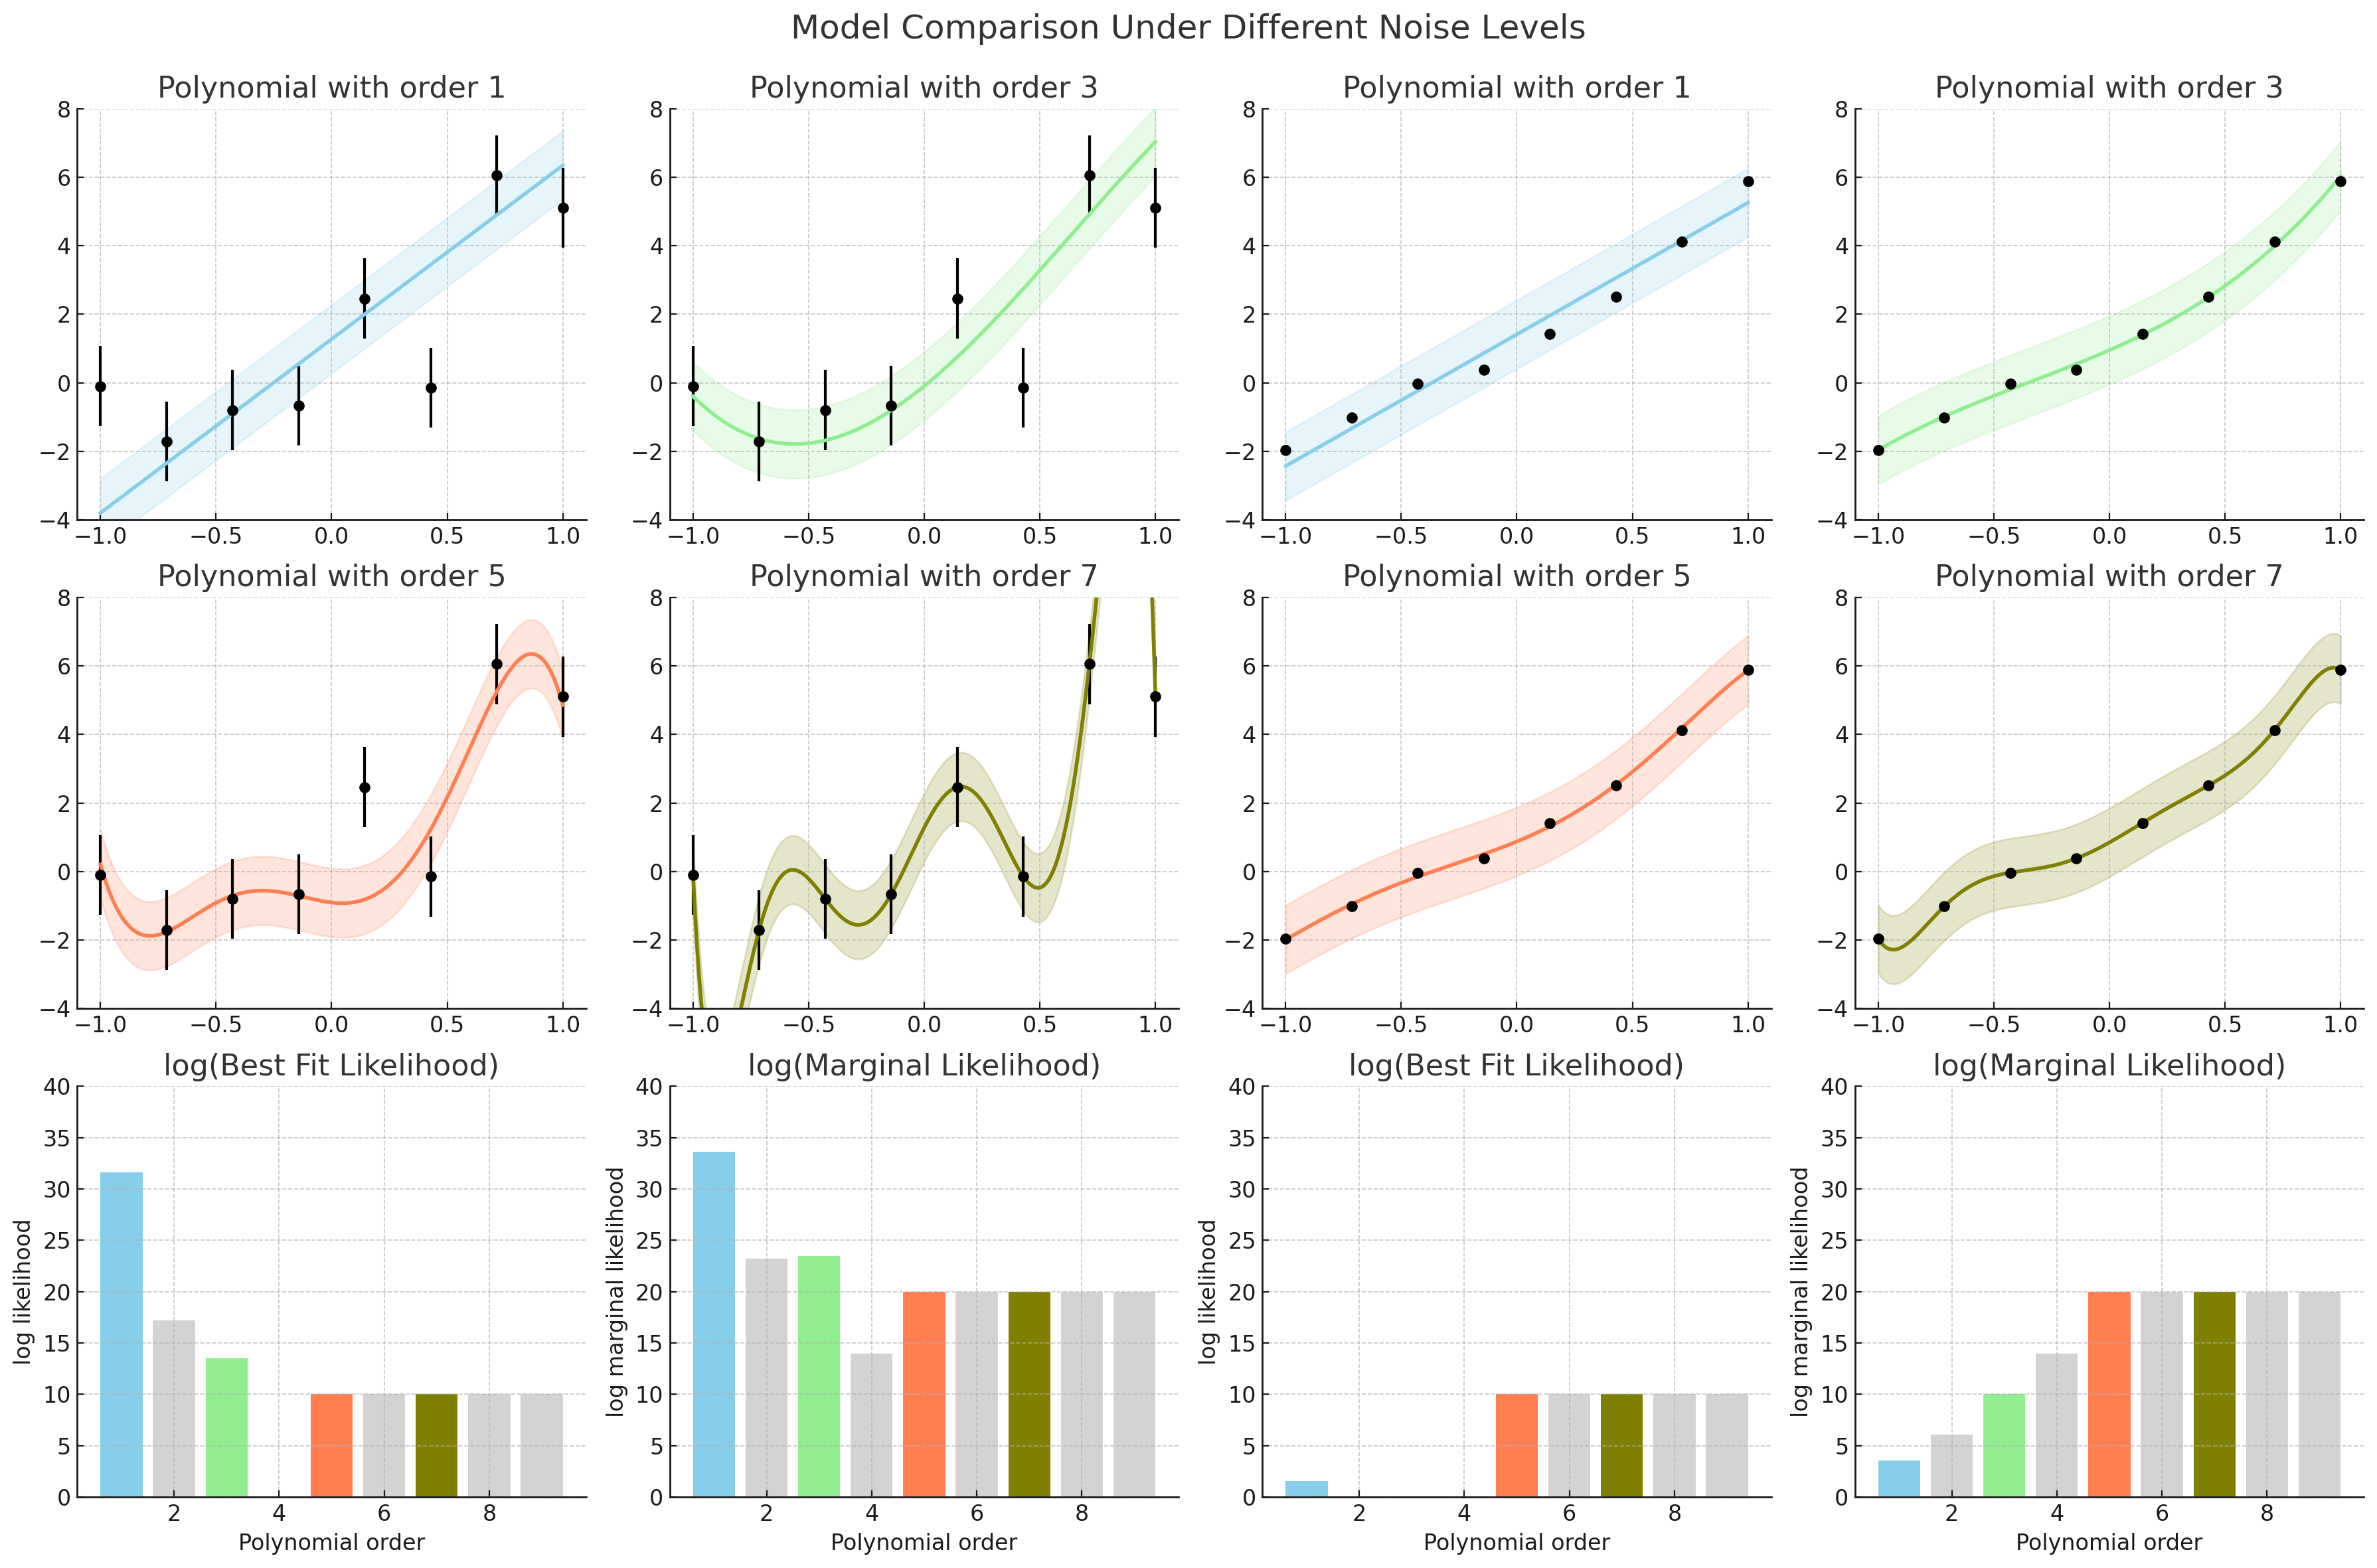
\includegraphics[width=0.9\linewidth]{MSc_Statistics_Research_Report_Template/images/output.png} 
\caption{ODR polynomial fits (orders 1, 3, 5, 7) to eight samples from a cubic ground truth under large (left) and small (right) noise. Bottom panels compare the marginal likelihood of different orders, where higher values indicate better model fit; the penalised score favours simpler models at high noise and selects order 3 at low noise.}
\end{figure}

One way to overcome this challenge is to make use of regression algorithms that account for the EIV.
Unlike ordinary least squares (OLS), which assumes error-free predictors, EIV algorithms explicitly account for measurement errors in both x and y, thereby mitigating attenuation bias in slope estimation \citep{fuller2009, carroll2006}. For nonlinear models, SINDy tries to learn one suitable candidate among EIV algorithms is Orthogonal Distance Regression (ODR).
ODR offer an effective way to explain these uncertainties on both sides of the regression equation \citep{boggs1989}. 
Empirical studies have shown that EIV-type estimators, such as Deming regression, principal component regression, and Bayesian EIV, provide less biased estimates than OLS in the presence of measurement errors \citep{mikkonen2019}. Comparative work has also highlighted the relative advantages of ODR and Bayesian EIV in geometric fitting tasks, such as circle and ellipse fitting, where ODR offers robust nonlinear extensions \citep{splett2018}. More recently, ODR has been incorporated into Bayesian model discovery frameworks, including SINDy, to improve robustness when both states and derivatives are noisy \citep{quade2018, champion2020}. Collectively, these contributions establish EIV and ODR as essential tools for handling measurement error in both predictors and responses across statistical modelling and data-driven scientific discovery.


\subsection{Contribution of this study}


This thesis introduces three novel model methods that can solve the selection of one-dimensional sparse polynomial models with noise. Because we aim to establish and validate the proposed methods in a controlled and transparent setting, so we consider the one-dimensional polynomial model as a simpler archetypal problem.

We develop a Bayesian evidence–based framework for sparse polynomial model selection that directly computes posterior model probabilities, thereby integrating Occam’s razor in a principled way. This approach enables model selection under the noise in the response variable, balancing fit and complexity without relying on asymptotic information criteria such as AIC or BIC. In doing so, it provides a fully probabilistic mechanism for identifying the most parsimonious model structure. 
In addition, we employ the SINDy methodology to mitigate the risk of overfitting in model selection under this setting, further enhancing interpretability and robustness.

To address the more challenging case where both predictors and responses are corrupted by measurement errors, we extend the SINDy framework by incorporating ODR. By coupling ODR with sequential thresholding, the proposed Sequentially Thresholded Least Squares with ODR (STLSQ-ODR) method explicitly corrects for EIV, yielding more robust coefficient estimates and enabling reliable recovery of governing equations under correlated and heavy-tailed noise.

Through simulation studies, we demonstrate the comparative advantages of each method under different noise structures and highlight the potential for future integration of Bayesian evidence with ODR-based sparsification to create a comprehensive noise-robust model selection framework.


\subsection{Structure of the paper}
The rest of this paper is organised as follows. In Section \ref{sec:meth}, we provide a detailed overview of the polynomial regression framework and its role in sparse model discovery. We first review the Bayesian razor method \citep{mackay2003}, which leverages Bayesian evidence and the Occam factor to balance model fit and complexity. This approach is easily applied in cases where noise is present only in the response variable, allowing for model selection among competing polynomial structures. We then introduce the STLSQ framework for model selection with noise in the response variable. Then we introduce the EIV problem that can be dealt with by 0ODR. We then introduce the STLSQ-ODR framework, which integrates sparse thresholded regression with ODR to explicitly account for measurement errors in both predictors and the response variable. Section \ref{sec:simu} presents empirical studies showcasing the performance of these three approaches under different noise structures and correlation settings, including both synthetic data experiments and robustness analyses. In Section \ref{sec:disc}, we compare the strengths and limitations of the three methods. Specifically, we discuss why the Bayesian razor excels in balancing model fit and complexity under moderate response noise, while the STLSQ-ODR method provides more robust estimation in scenarios where measurement errors occur in both inputs and outputs. Finally, we conclude with remarks on potential extensions and future research directions, including the integration of Bayesian evidence with ODR-based sparsification to enable more comprehensive model selection.
\section{Methodology}
\label{sec:meth}


This section proposes establishing a model selection framework for the one-dimensional polynomial model in two different scenarios. 
First, when noise is present only in the response variable, we address model selection using the Bayesian razor and SINDy approaches. Second, when noise affects both the predictors and the response, we employ the STLSQ–ODR framework to account explicitly for EIV problem.

\subsection{Add the noise just in the response variable}
\label{subsec:noise_y}

The polynomial model with noise in the response variable is:
\begin{equation} 
\label{eq:modely_1}
y_i = f(\boldsymbol{x_i}) + \varepsilon_i, \quad  \varepsilon_i \overset{\mathrm{i.i.d.}}{\sim} \mathcal{N}(0, \sigma^2), \quad i = 1 \ldots N
\end{equation}
where $f(x) = \alpha_0 + \alpha_1\boldsymbol{x}+\alpha_2\boldsymbol{x}^2+ \ldots + \alpha_n\boldsymbol{x}^n$. Or equivalently in matrix form:
\begin{equation} 
\label{eq:modely_2}
\boldsymbol{y} = \mathbf{\Phi} \boldsymbol{w} + \boldsymbol{\varepsilon}, \qquad \boldsymbol{\varepsilon} \sim \mathcal{N}(0, \boldsymbol{\Sigma})
\end{equation}
where the design matrix and the basis functions are $\mathbf{\Phi} = \big(\phi(\boldsymbol{x_{1}})^{\mathsf{T}} \ldots\phi(\boldsymbol{x_{N}})^{\mathsf{T}}\big)^{\mathsf{T}}, 
\phi(\boldsymbol{x})= (\boldsymbol{1}\ \boldsymbol{x} \ \boldsymbol{x}^{2} \ldots \boldsymbol{x}^{n})^{\mathsf{T}},$ and the off-diagonal entries of $\boldsymbol{\Sigma}$ are zero, such that we can denote $\boldsymbol{\Sigma} = (\rho_{ij})_{i,j=1}$ with $\rho_{ij} = 0$ for $i \neq j$. Assume that that the prior distribution of $\boldsymbol{w}$ follows the Gaussian distribution, that is $\boldsymbol{w} \sim \mathcal{N}(\mathbf{0}, \mathbf{\Lambda}_0^{-1}).$ 
By virtue of the fact that a Gaussian distribution is closed under linear transformations, the distribution of the likelihood is still the Gaussian distribution: $p(\boldsymbol{y} \mid \boldsymbol{w}) = \mathcal{N}(\mathbf{\Phi} \boldsymbol{w}, \sigma^2 \mathbf{I})$.
Using Gaussian approximations for the prior and likelihood can speed up computation.

From Bayes’ rule, the posterior distribution of $p(\boldsymbol{w} \mid \boldsymbol{y}, \boldsymbol{\Phi}, \sigma^2, \boldsymbol{\Lambda}_0)$ can be expressed as being proportional to the product of the prior and the likelihood function: 
\begin{equation}
    p(\boldsymbol{w}\mid \boldsymbol{y}, \boldsymbol{\Phi}, \sigma^2, \boldsymbol{\Lambda}_0) \propto p(\boldsymbol{y}\mid \boldsymbol{w}, \boldsymbol{\Phi}, \sigma^2, \boldsymbol{\Lambda}_0) \, p(\boldsymbol{w}\mid \boldsymbol{\Phi}, \sigma^2, \boldsymbol{\Lambda}_0).
\end{equation}
Writing out the log posterior:
\begin{equation}
    \begin{aligned}
\log p(\boldsymbol{w}\mid \boldsymbol{y}, \boldsymbol{\Phi}, \sigma^2, \boldsymbol{\Lambda}_0) = \; & 
- \frac{1}{2 \sigma^2} \| \boldsymbol{y} - \mathbf{\Phi} \boldsymbol{w} \|^2
- \frac{1}{2} \boldsymbol{w}^\mathsf{T} \mathbf{\Lambda}_0 \boldsymbol{w} + C \\
=\; &
- \frac{1}{2 \sigma^2} \left( \boldsymbol{y}^\mathsf{T} \boldsymbol{y} 
- 2 \boldsymbol{w}^\mathsf{T} \mathbf{\Phi}^\mathsf{T} \boldsymbol{y} 
+ \boldsymbol{w}^\mathsf{T} \mathbf{\Phi}^\mathsf{T} \mathbf{\Phi} \boldsymbol{w} \right) 
- \frac{1}{2} \boldsymbol{w}^\mathsf{T} \mathbf{\Lambda}_0 \boldsymbol{w} + C.
\end{aligned}
\end{equation}

Grouping of quadratic and linear terms:
\begin{equation}
\label{log}
    \begin{aligned}
\log p(\boldsymbol{w} \mid \boldsymbol{y})
& =
    -\frac{1}{2}
    \boldsymbol{w}^\mathsf{T}
    \left( \sigma^{-2} \boldsymbol{\Phi}^\mathsf{T} \boldsymbol{\Phi} + \boldsymbol{\Lambda}_0 \right)
    \boldsymbol{w}
    + \boldsymbol{w}^\mathsf{T}
    \sigma^{-2} \boldsymbol{\Phi}^\mathsf{T} \boldsymbol{y} + C
\\
& =
    -\frac{1}{2}
    (\boldsymbol{w} - \boldsymbol{\mu})^\mathsf{T} \left( \sigma^{-2} \boldsymbol{\Phi}^\mathsf{T} \boldsymbol{\Phi} + \boldsymbol{\Lambda}_0 \right) (\boldsymbol{w} - \boldsymbol{\mu})
    - \boldsymbol{w}^\mathsf{T} \left( \sigma^{-2} \boldsymbol{\Phi}^\mathsf{T} \boldsymbol{\Phi} + \boldsymbol{\Lambda}_0 \right) \boldsymbol{\mu} \\
&     + \boldsymbol{w}^\mathsf{T} \sigma^{-2} \boldsymbol{\Phi}^\mathsf{T} \boldsymbol{y} + C.
\end{aligned}
\end{equation}
Inspection of the quadratic term reveals that the covariance matrix of the posterior distribution is
\begin{equation}
\label{covariance}
    \boldsymbol{\Sigma} = \left( \sigma^{-2} \boldsymbol{\Phi}^\mathsf{T} \boldsymbol{\Phi} + \boldsymbol{\Lambda}_0 \right)^{-1}.
\end{equation}
So (\ref{log}) can be written as
\begin{equation}
    \log p(\boldsymbol{w} \mid \boldsymbol{y}) = -\frac{1}{2}
    (\boldsymbol{w} - \boldsymbol{\mu})^\mathsf{T} \Sigma^{-1} (\boldsymbol{w} - \boldsymbol{\mu})
    - \boldsymbol{w}^\mathsf{T} \Sigma^{-1} \boldsymbol{\mu}
    + \boldsymbol{w}^\mathsf{T} \sigma^{-2} \boldsymbol{\Phi}^\mathsf{T} \boldsymbol{y} + C.
\end{equation}
Given that $\boldsymbol{w}^\mathsf{T} \boldsymbol{\Sigma}^{-1} \boldsymbol{\mu}
    + \boldsymbol{w}^\mathsf{T} \sigma^{-2} \boldsymbol{\Phi}^\mathsf{T} \boldsymbol{y} = 0$, that we need $\boldsymbol{\Sigma}^{-1} \boldsymbol{\mu} = \sigma_n^{-2} \boldsymbol{\Phi}^\mathsf{T} \boldsymbol{y}$,
It follows that the mean of the posterior distribution is
\begin{equation}
\label{mean}
    \boldsymbol{\mu} = \boldsymbol{\Sigma} \left( \sigma_n^{-2} \boldsymbol{\Phi}^\mathsf{T} \boldsymbol{y} \right).
\end{equation}
In summary, the posterior distribution is Gaussian with
\begin{equation}
    p(\boldsymbol{w}\mid \boldsymbol{y}, \boldsymbol{\Phi}, \sigma^2, \boldsymbol{\Lambda}_0) \propto\ \mathcal{N}(\boldsymbol{\mu}, \boldsymbol{\Sigma}).
\end{equation}
with $\boldsymbol{\mu}$ and $\boldsymbol{\Sigma}$ given by (\ref{mean}) and (\ref{covariance}).

\subsubsection{The Mechanism of the Bayesian Razor: the Bayesian Evidence \& Occam Factor}

This approach is grounded in the principle that Bayesian inference naturally balances model fit with model complexity through the Occam factor, thereby avoiding overfitting in polynomial model selection. 
Specifically, under the assumption of a Gaussian prior distribution over model parameters, the Bayesian razor evaluates the marginal likelihood of each candidate polynomial model, penalizing unnecessarily complex models that do not substantially improve the data likelihood. 
In contrast to classical information criteria such as AIC or BIC, which rely on asymptotic approximations, the Bayesian razor provides a fully probabilistic and principled framework that explicitly integrates uncertainty in both model parameters and data noise. 

Bayesian inference offers a principled framework for model comparison that naturally incorporates Occam's razor, the preference for simpler models that sufficiently explain the data. The plausibility of a model $\mathrm{H}_i$ is quantified by its posterior probability:
\begin{equation}
\mathbb{P}(\mathrm{H}_i \mid \mathbf{D}) \propto \mathbb{P}(\mathbf{D} \mid \mathrm{H}_i) \mathbb{P}(\mathrm{H}_i),
\end{equation}
where $\mathbb{P}(\mathrm{H}_i)$ is the prior model probability and $\mathbb{P}(\mathbf{D} \mid \mathrm{H}_i)$ is the Bayesian evidence (marginal likelihood).

\paragraph{Two levels of inference.}
\begin{enumerate}
    \item \textbf{Model fitting:} For a given model $\mathrm{H}_i$ with
    parameters $\boldsymbol{w}$,
    \begin{equation}
    p(\boldsymbol{w} \mid \mathbf{D}, \mathrm{H}_i) =
    \frac{p(\mathbf{D} \mid \boldsymbol{w}, \mathrm{H}_i) p(\boldsymbol{w} \mid \mathrm{H}_i)}{p(\mathbf{D} \mid \mathrm{H}_i)},
    \end{equation}
    where $p(\mathbf{D}\mid \boldsymbol{w}, \mathrm{H}_i)$ is the likelihood and $p(\boldsymbol{w} \mid \mathrm{H}_i)$
    the parameter prior. The denominator $p(\mathbf{D} \mid \mathrm{H}_i)$ is the evidence, often
    ignored in parameter estimation but essential for model comparison.

    \item \textbf{Model comparison:} Models are ranked by their evidences,
    assuming equal model priors:
    \begin{equation}
    p(\mathbf{D} \mid \mathrm{H}_i) = \int p(\mathbf{D} \mid \boldsymbol{w}, \mathrm{H}_i) p(\boldsymbol{w} \mid \mathrm{H}_i) \, d\boldsymbol{w}.
    \end{equation}
    Complex models with larger parameter spaces dilute their predictive probability
    over more possibilities, resulting in a natural penalty.
\end{enumerate}

\paragraph{Evidence decomposition and Occam factor.}
When the posterior is sharply peaked at the maximum a posteriori estimate
$\boldsymbol{w}_{\mathrm{MAP}}$, Laplace's method yields:
\begin{equation}
p(\mathbf{D} \mid \mathrm{H}_i) \approx p(\mathbf{D} \mid \boldsymbol{w}_{\mathrm{MAP}}, \mathrm{H}_i) \times
\frac{\sigma_{\boldsymbol{w} \mid \mathbf{D}}}{\sigma_{\boldsymbol{w}}},
\end{equation}
where $\sigma_{\boldsymbol{w}}$ and $\sigma_{\boldsymbol{w} \mid \mathbf{D}}$ denote the prior and
posterior widths of the parameter space, respectively.
The second factor,
\begin{equation}
\mathrm{Occam\ factor} = \frac{\sigma_{\boldsymbol{w} \mid \mathbf{D}}}{\sigma_{\boldsymbol{w}}},
\end{equation}
penalizes models whose parameter space must be finely tuned to fit the data.
In the multi-parameter case, the Occam factor generalizes to:
\begin{equation}
p(\mathbf{D} \mid \mathrm{H}_i) \approx p(\mathbf{D} \mid \boldsymbol{w}_{\mathrm{MAP}}, \mathrm{H}_i) \,
p(\boldsymbol{w}_{\mathrm{MAP}} \mid \mathrm{H}_i) \,
\det\nolimits^{-1/2}\!\left(\frac{\mathbf{A}}{2\pi}\right),
\end{equation}
where $\mathbf{A}$ is the Hessian of the negative log posterior.

Laplace approximation about the MAP point
yields
\[
\log p(\mathbf{D} \mid \mathrm{H}_i) \approx
\underbrace{\log p(\mathbf D \mid \boldsymbol{w}_{\mathrm{MAP}},\mathrm{H}_i)}_{\text{Likelihood at MAP}}
+
\underbrace{\log p(\boldsymbol{w}_{\mathrm{MAP}}\mid \mathrm{H}_i) - \frac{1}{2} \log\det\left( \frac{\bf{A}}{2\pi}\right),}_{\text{Occam factor}}
\]
where
$\bf{A} \;=\; \bf{\Lambda}_{\text{post}}
       = \mathbf{\Lambda}_0 + \boldsymbol{\beta} \Phi^{\!\top} \Phi,
\bf{\Sigma}_{\text{post}} = \bf{A}^{-1},  
\boldsymbol{w}_{\mathrm{MAP}}
       = \bf{\Sigma}_{\text{post}}
         \bigl(\mathbf{\Lambda}_0 \boldsymbol\mu_0 + \boldsymbol{\beta} \Phi^{\!\top} \mathbf t \bigr).$

\smallskip
\begin{itemize}\setlength\itemsep{2pt}
  \item Best–Fit Likelihood captures how well the model fits the data at the MAP parameters.
  \item Occam factor penalises model complexity via $\det \mathbf{A}$: the narrower the posterior, the larger the penalty.
\end{itemize}

However, extending the Bayesian razor framework to the error-in-variable (EIV) problem is highly challenging. The main difficulty arises because EIV models fundamentally alter the likelihood structure. The observed predictors no longer represent the true regressors, leading to attenuation bias and complex error propagation through nonlinear basis functions. As a consequence, the marginal likelihood integral required by the Bayesian razor becomes analytically intractable, since it must integrate over both latent clean predictors and model parameters simultaneously. This dramatically increases computational cost and introduces severe identifiability issues, as different combinations of latent predictor distributions and polynomial structures may yield similar fits to noisy data. 
To address this difficulty, we turn to ODR, which provides a principled way to handle measurement errors in both predictors and responses.

\subsubsection{The Mechanism of the STLSQ}
Since implementing full Bayesian model selection is difficult when solving the EIV problem, we resort to simpler, sparsity-inducing alternatives that thereby approximate Occam’s razor.
Within the SINDy framework, the STLSQ algorithm serves as an alternative, computationally efficient approach to induce sparsity, offering a simpler substitute to more elaborate Bayesian selection methods.
The STLSQ algorithm is the standard regression procedure employed in the SINDy framework to enforce sparsity in the model selection process (\cite{brunton2016}). Its primary objective is to identify a parsimonious subset of active basis functions from a potentially large candidate library $\mathbf{\Phi}(x)$. Consider observations $\boldsymbol{y} \in \mathbb{R}^n$ and the design matrix $\mathbf{\Phi} \in \mathbb{R}^{n \times p}$ constructed from polynomial basis functions. The regression model is same as equation  (\ref{eq:modely_2}).

The STLSQ algorithm alternates between two steps:
\begin{itemize}
    \item \textbf{Least-squares update:} Solve the ordinary least squares problem
    \begin{equation}
\hat{\boldsymbol{w}} = \arg\min_{\boldsymbol{w}} \|\boldsymbol{y} - \mathbf{\Phi} \boldsymbol{w}\|_2^2,
\end{equation}
to obtain coefficient estimates.
    \item \textbf{Thresholding:} Apply a sparsity threshold $\lambda > 0$ to eliminate coefficients whose magnitude falls below the threshold:
\begin{equation}
\hat{w}_j \leftarrow 0 \quad \text{if} \quad |\hat{w}_j| < \lambda.
\end{equation}
\end{itemize}

This two-step procedure is repeated iteratively until convergence. The mechanism ensures that small, noise-dominated coefficients are discarded while retaining only the dominant terms that capture the essential dynamics of the system. 
In this way, STLSQ prevents overfitting by balancing model fit with parsimony, thereby providing interpretable models that generalise well. Much like Bayesian evidence, it can be regarded as applying the principle of Occam’s razor, but without computing the posterior distribution, which makes it considerably simpler and more computationally efficient.



\subsection{Add the noise in both predictor variables and response variable}
\label{subsec:noise_xy}

\subsubsection{The basic principles of ODR}
Let $\{(\boldsymbol{x}_i,y_i)\}_{i=1}^n$ be observed data, with $\boldsymbol{x}_i\in\mathbb{R}^m$ and scalar response $y_i$.
We posit a smooth model $y = f(\boldsymbol{x};\boldsymbol{\beta})$ with parameter vector $\boldsymbol{\beta}\in\mathbb{R}^p$.
Unlike ordinary least squares (OLS), which assumes errors only in $y$, ODR allows measurement errors in both the response and the predictors. We write
\begin{equation}
    y_i = f(\boldsymbol{x}_i+\boldsymbol{\delta}_i;\,\boldsymbol{\beta})\;-\;\varepsilon_i,
\end{equation}
where $\varepsilon_i$ is the additive error in the response and $\boldsymbol{\delta}_i\in\mathbb{R}^m$ is the additive error (adjustment) in the predictors.


Define the orthogonal distance of the point $(\boldsymbol{x}_i,y_i)$ to the model as $r_i^2 \;=\; \varepsilon_i^2 \;+\; \|\boldsymbol{\delta}_i\|_2^2.$
Minimising the sum of squared distances subject to the model relation
\begin{equation}
    \min_{\boldsymbol{\beta},\;\{\varepsilon_i,\boldsymbol{\delta}_i\}}\;\sum_{i=1}^n r_i^2,
\end{equation}
same as the unconstrained problem
\begin{equation}
\min_{\boldsymbol{\beta},{\boldsymbol{\delta}_i}} \;\sum_{i=1}^n \Big\{( f(\boldsymbol{x}_i+\boldsymbol{\delta}_i;\boldsymbol{\beta}) - y_i )^2 \;+\; \|\boldsymbol{\delta}_i\|_2^2\Big\}.
\end{equation}
In ODR, the optimal parameters $\hat{\boldsymbol{\beta}}$ minimize the sum of squared orthogonal distances from the observed points $(\boldsymbol{x}_i, y_i)$ to the model curve $f(\cdot; \boldsymbol{\beta})$, leading to the optimization problem
\begin{equation}
    \min_{\boldsymbol{\beta}, \boldsymbol{\delta}_i} \sum_{i=1}^n \left[ f(\boldsymbol{x}_i+\boldsymbol{\delta}_i; \boldsymbol{\beta}) - y_i \right]^2
+ d_i^2 \boldsymbol{\delta}_i^2,
\end{equation}
where $d_i = \sigma_\epsilon / \sigma_\delta$ and $w_i = 1 / \sigma_\epsilon$ are weights.




\subsection{The Mechanism of the STLSQ\_ODR}

For the model which adds noise in both predictor variables and the response variable, we combine the SINDy framework with ODR.
ODR explicitly accounts for errors in both the predictors and the response by minimizing the scaled orthogonal distance from noisy observations to the model manifold, thus providing de-noised inputs and more reliable regression estimates. 
Within our framework, the SINDy algorithm first constructs a candidate library of nonlinear functions of the state variables, while ODR is employed to perform sparse regression under an errors-in-variables setting. This joint approach allows us to recover the correct governing equations even in the presence of correlated noise in both predictors and responses, improving robustness compared with standard SINDy.



To ensure numerical stability across polynomial orders, we normalise each basis function using its $L^2([-1,1])$ norm,
\begin{equation}
    \mathrm{factor}[k] = \sqrt{\frac{2k+1}{2}}, \quad k=0,1,\dots,d,
\end{equation}
and perform regression in the normalised basis. Since the sparsity threshold $\lambda$ is applied uniformly across all coefficients, the scaling of the basis directly affects whether terms are eliminated or retained. Without normalization, higher-order terms may appear artificially large and survive the thresholding step, while lower-order terms may be prematurely discarded. By applying the $L^2([-1,1])$ normalization, we ensure that the thresholding operates on a balanced scale across all polynomial orders, thereby improving the robustness of sparse model selection. 

Given observed predictors $x \in \mathbb{R}^n$ and response $\dot{x} \in \mathbb{R}^n$, ODR estimates the coefficient vector $\hat{w}$ by solving
\begin{equation}
    \hat{\boldsymbol{w}} = \arg\min_{\boldsymbol{w},\,\boldsymbol{\delta}_i} \sum_{i=1}^n \left( \dot{\boldsymbol{x}}_i - \mathbf{\Phi}(\boldsymbol{x}_i + \boldsymbol{\delta}_i)\boldsymbol{w} \right)^2 + \|\boldsymbol{\delta}_i\|_2^2,
\end{equation}
where $\boldsymbol{\delta}_i$ denotes the adjustment to noisy predictors. 

The Sequential Thresholded step is then applied on the normalized coefficients:  
\begin{equation}
    \hat{w}_j \leftarrow 0 \quad \text{if} \quad |\hat{w}_j| < \lambda,
\end{equation}
with $\lambda > 0$ a sparsity threshold. The regression is subsequently refitted on the retained terms, and this two-step procedure is iterated until convergence. Finally, the coefficients are denormalised back to the standard polynomial scale:
\begin{equation}
    w_j = \hat{w}_j \cdot \mathrm{factor}[j], \quad j=0,1,\dots,d.
\end{equation}

This iterative procedure, which we term STLSQ-ODR, integrates the mechanism of SINDy with ODR. As a result, the method yields sparse yet robust recovery of governing equations, even in the presence of correlated noise in both predictors and responses.



\section{Simulation Studies}
\label{sec:simu}

This section presents simulation studies to examine the empirical performance of the proposed model selection frameworks under different noise settings. 
In Section \ref{subsec:study1} and \ref{subsec:STLSQ}, we investigate the Bayesian Razor method and STLSQ algorithm for polynomial regression models with noise only in the response variable. 
In Section \ref{subsec:study2}, we evaluate the STLSQ-ODR procedure for polynomial regression models with noise in both predictors and responses, considering Gaussian, Student-t, and correlated noise structures. Across all experiments, we generate synthetic datasets from polynomial ground truth models, systematically vary the noise levels, and assess model recovery accuracy in terms of posterior probabilities and sparse coefficient estimation.

\subsection{Study 1: Bayesian Razor Method Evidence}
\label{subsec:study1}

This subsection conducts the empirical performance of Bayesian Razor for a polynomial regression model with added noise in the response variable. 
Specifically, we consider a univariate polynomial regression setting, where the true data-generating function is a cubic polynomial given by $y = 3 - 2x + x^3$ with additive Gaussian noise $\varepsilon_i \sim \mathcal{N}(0, \sigma^2)$ in $y$, where $\sigma = 0.1, 0.3,0.5$. We use $n=1000$ evenly spaced input points over $[-1, 1]$ to simulate a low-data regime.

To explore the performance of Bayesian model selection under limited data, we evaluate all $2^4 - 1 = 15$ non-empty subsets of candidate polynomial basis functions ${1, x, x^2, x^3}$. For each subset, we compute the MAP estimate of the regression coefficients under a zero-mean Gaussian prior with unit variance, and calculate the marginal likelihood (evidence) assuming a fixed likelihood precision.


The posterior probability of each model is computed by normalising its marginal likelihood across all models. We then compare these models in terms of both their posterior probability and coefficient estimates, ultimately identifying the model with the highest posterior probability. 

\begin{figure}[htbp]
\centering
\begin{minipage}{0.47\textwidth}
    \centering
    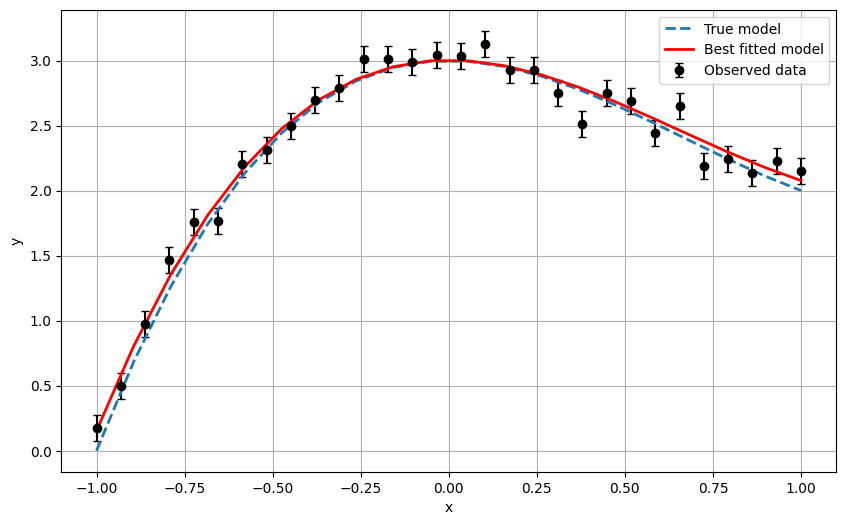
\includegraphics[width=\linewidth]{MSc_Statistics_Research_Report_Template/images/n=30, sigma=0.1.png}
    \subcaption{$n=30$, $\sigma=0.1$}
\end{minipage}
\begin{minipage}{0.47\textwidth}
    \centering
    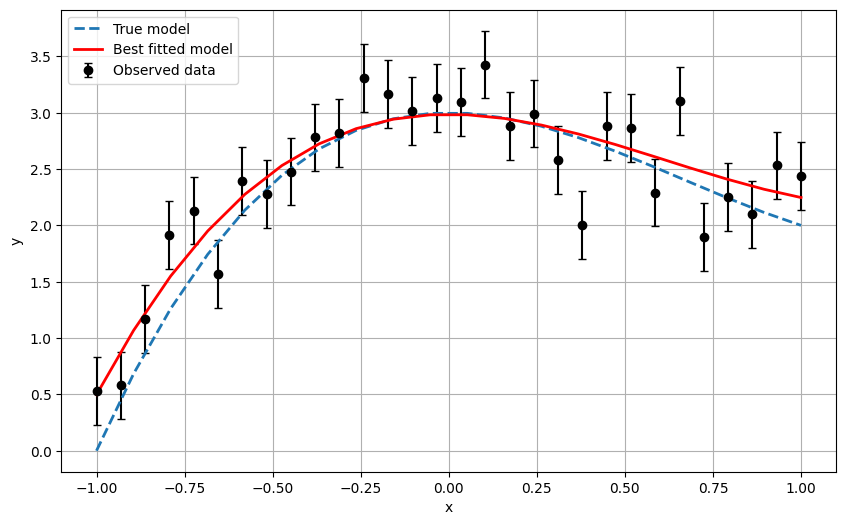
\includegraphics[width=\linewidth]{MSc_Statistics_Research_Report_Template/images/n=30, sigma=0.3.png}
    \subcaption{$n=30$, $\sigma=0.3$}
\end{minipage}
\begin{minipage}{0.47\textwidth}
    \centering
    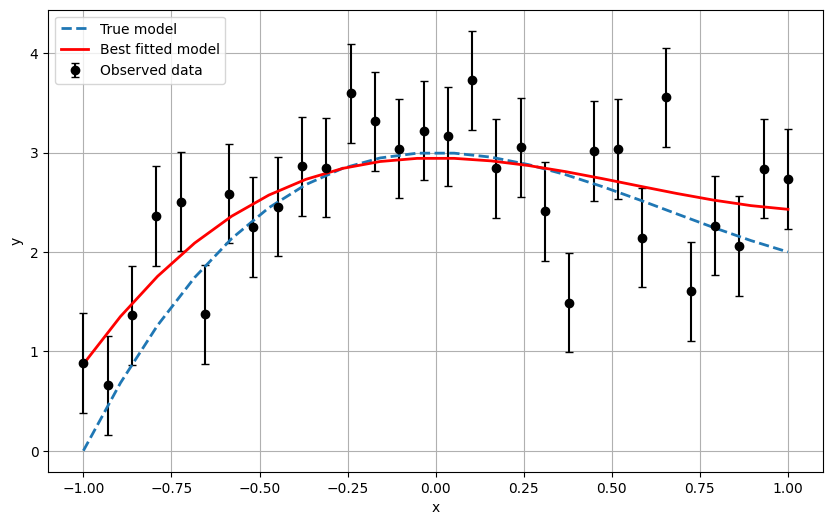
\includegraphics[width=\linewidth]{MSc_Statistics_Research_Report_Template/images/n=30, sigma=0.5.png} 
    \subcaption{$n=30$, $\sigma=0.5$}
\end{minipage}
\begin{minipage}{0.47\textwidth}
    \centering
    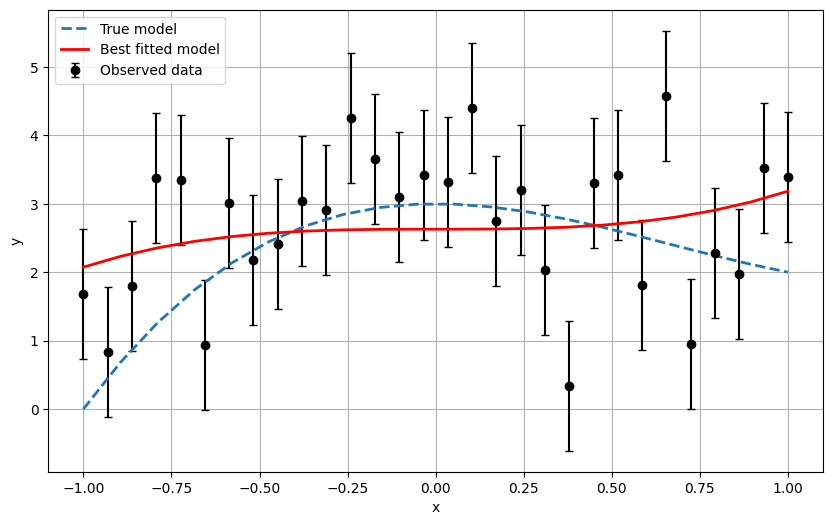
\includegraphics[width=\linewidth]{MSc_Statistics_Research_Report_Template/images/n=30, sigma=0.95.png}
    \subcaption{$n=30$, $\sigma=0.95$}
\end{minipage}
\caption{Comparison of the true model, best fitted model, and observed data with different error bars.}
\label{fig:n=30}
\end{figure}

Table \ref{tab:Bayesian_Razor} presents the simulation outcomes under different noise variance settings. Under moderate noise levels, the Bayesian razor method efficiently and accurately identifies the polynomial terms and provides good estimates of their corresponding coefficients. As the noise variance increases from $0.1$ to $3.0$, both the accuracy of coefficient estimation and the posterior probability of selecting the correct model exhibit a slight decline. Nevertheless, the Bayesian\_razor method still maintains strong model selection performance. 
When the observation noise exceeds approximately 
$\sigma \approx 3.9$, the Bayesian Razor method selects an oversimplified and incorrect polynomial model, indicating model failure. 
This breakdown occurs because the noise overwhelms the signal, and the 
marginal likelihood, through Occam's penalty, favours lower-complexity 
models, thereby leading to underfitting.

\begin{table}
\centering
\caption{Posterior probability of Bayesian Razor Method under varying noise levels $\sigma$} 
\label{tab:Bayesian_Razor} 
\begin{tabular}{cccc}
\toprule
$\sigma$ & Model ($\mathrm{H}_i$) & Posterior Probability & $\boldsymbol{w}_{\mathrm{MAP}}$ \\
\midrule
0.1 & $\mathbf{x^3, x^2, 1}$ & \textbf{0.986} & $(1.000,\,-1.967,\,2.985)$ \\
    & $x^3, x^2, x^1, 1$     & 0.014          & $(1.006,\,-1.967,\,-0.004,\,2.985)$ \\
\midrule
0.5 & $\mathbf{x^3, x^2, 1}$ & \textbf{0.935} & $(0.997,\,-1.831,\,2.920)$ \\
    & $x^3, x^2, x^1, 1$     & 0.065          & $(1.019,\,-1.831,\,-0.016,\,2.920)$ \\
\midrule
1.0 & $\mathbf{x^3, x^2, 1}$ & \textbf{0.881} & $(0.990,\,-1.648,\,2.834)$ \\
    & $x^3, x^2, x^1, 1$    & 0.119          & $(1.015,\,-1.648,\,-0.018,\,2.834)$ \\
\midrule
2.0 & $\mathbf{x^3, x^2, 1}$ & \textbf{0.785} & $(0.966,\,-1.258,\,2.651)$ \\
    & $x^3, x^2, x^1, 1$    & 0.195          & $(0.954,\,-1.258,\,0.009,\,2.651)$ \\
    & $x^2, x^1, 1$          & 0.020          & $(-1.258,\,0.576,\,2.651)$ \\
\midrule
3.0 & $\mathbf{x^3, x^2, 1}$ & \textbf{0.629} & $(0.931,\,-0.861,\,2.462)$ \\
    & $x^3, x^2, x^1, 1$    & 0.215          & $(0.857,\,-0.861,\,0.057,\,2.462)$ \\
    & $x^2, x^1, 1$          & 0.101          & $(-0.861,\,0.558,\,2.462)$ \\
    & $x^3, 1$                & 0.035          & $(0.931,\,2.177)$ \\
    & $x^3, x^1, 1$          & 0.012          & $(0.857,\,0.057,\,2.177)$ \\
    & $x^1, 1$                & 0.006          & $(0.558,\,2.177)$ \\
    & $x^2, 1$                & 0.002          & $(-0.861,\,2.462)$ \\
\midrule    
3.9 & $\mathbf{x^3, 1}$       & \textbf{0.287} & $(0.892,\,2.123)$ \\
    & $x^3, x^2, 1$          & 0.280          & $(0.892,\,-0.521,\,2.295)$ \\
    & $x^3, x^1, 1$          & 0.118          & $(0.766,\,0.100,\,2.123)$ \\
    & $x^3, x^2, x^1, 1$    & 0.115          & $(0.766,\,-0.521,\,0.100,\,2.295)$ \\
    & $x^1, 1$                & 0.086          & $(0.540,\,2.123)$ \\
    & $x^2, x^1, 1$          & 0.084          & $(-0.521,\,0.540,\,2.295)$ \\
    & $1$                      & 0.015          & $(2.123)$ \\
    & $x^2, 1$                & 0.014          & $(-0.521,\,2.295)$ \\
\bottomrule
\end{tabular}
\end{table}

Figure \ref{fig:true_vs_fitted} illustrates the comparison between the true polynomial model and the best fitted model obtained under different noise variances. The fitted curve remains close to the true model when the noise variance is relatively small ($\sigma^2 = 0.5$ or $\sigma^2 = 1.0$). However, as the variance increases, the discrepancy between the fitted and true curves becomes more pronounced. In particular, for larger noise levels ( $\sigma^2 = 2.0$ and $\sigma^2 = 3.0$), the fitted model fails to capture the underlying polynomial structure accurately, exhibiting systematic deviations from the true curve. This observation highlights the sensitivity of the model selection procedure to the signal-to-noise ratio: while reliable recovery of the true structure is feasible under moderate noise, excessive noise leads to model misspecification and underfitting.


\begin{figure}
\centering
\setlength{\tabcolsep}{2pt} % 图之间的水平间距
\renewcommand{\arraystretch}{0.5} % 控制行距
\begin{tabular}{@{}cc@{}}
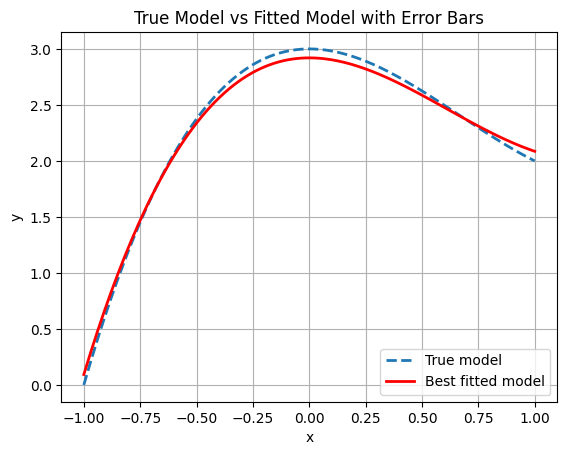
\includegraphics[width=0.48\textwidth]{MSc_Statistics_Research_Report_Template/images/sigma0.5.png} &
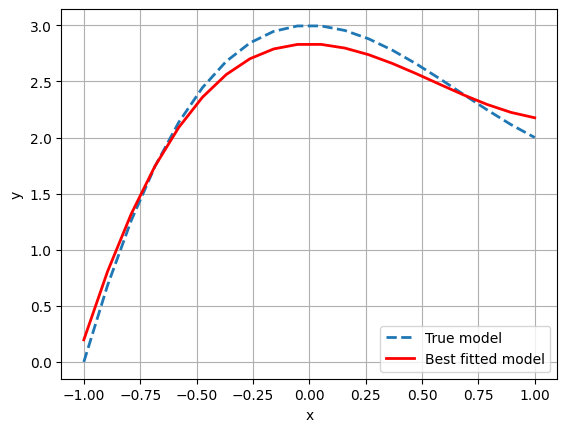
\includegraphics[width=0.48\textwidth]{MSc_Statistics_Research_Report_Template/images/sigma1.0.png} \\
\small (a) $\sigma^2=0.5$ & \small (b) $\sigma^2=1.0$ \\
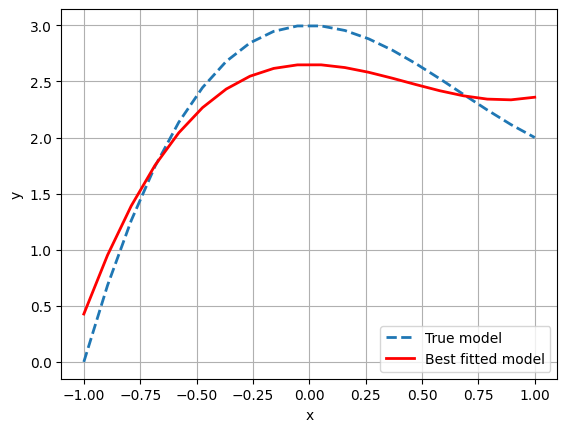
\includegraphics[width=0.48\textwidth]{MSc_Statistics_Research_Report_Template/images/sigma2.0.png} &
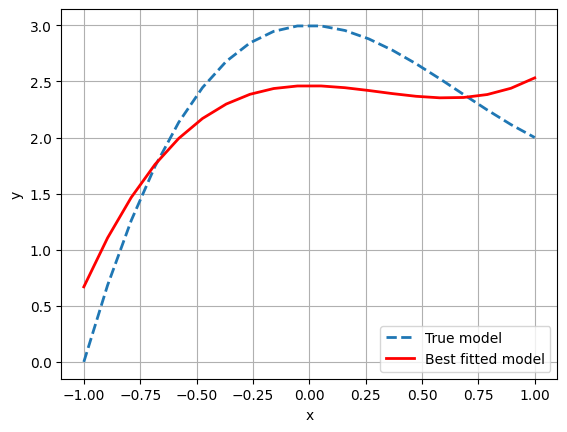
\includegraphics[width=0.48\textwidth]{MSc_Statistics_Research_Report_Template/images/sigma3.0.png} \\
\small (c) $\sigma^2=2.0$ & \small (d) $\sigma^2=3.0$
\end{tabular}
\caption{Comparison of the true model and best fitted model under different noise variances.}
\label{fig:true_vs_fitted}
\end{figure}







\subsection{Study 2: STLSQ Framework}
\label{subsec:STLSQ}
This subsection investigates the performance of the STLSQ method for polynomial regression with additive noise in the response variable. In particular, we study a univariate regression problem where the true underlying model is the sixth-order polynomial $y = 3 - 2x + 0.5x^3 + x^5,$
corrupted by additive Gaussian noise $\varepsilon_i \sim \mathcal{N}(0, 0.05^2)$. We generate $n=1000$ evenly spaced design points over the interval $[-1,1]$ and construct the corresponding polynomial feature library up to degree five. 

To evaluate the effectiveness of sparse regression, we compare two approaches for selecting the sparsity threshold $\lambda$. \begin{itemize}
\item Method 1: The sparsity threshold $\lambda$ is selected by first performing OLS regression and identifying the smallest non-zero coefficient in magnitude. We then set:
$\lambda = 0.9 \times \min(|\text{non-zero OLS coefficients}|).$

The smallest non-zero coefficient from the OLS fit can be regarded as the weakest yet still relevant feature. If the threshold were set exactly equal to this value, the corresponding coefficient would be eliminated during sparsification, potentially removing a meaningful feature. Multiplying by 0.9 lowers the threshold slightly below this boundary, thereby preserving the smallest coefficient while discarding smaller noise-dominated terms. This scaling factor mitigates the risk of erroneous elimination caused by numerical rounding or fluctuations in noisy data.
\item Method 2: Grid-search with BIC: 
We perform a grid search over logarithmically spaced values of $\lambda$ with the optimal value determined by minimising the BIC:
\begin{equation}
    \mathrm{BIC} = n \ln\!\left(\frac{\mathrm{RSS}}{n}\right) + k \ln(n),
\end{equation}
where $\mathrm{RSS}_{\text{STLSQ}}
= \sum_{i=1}^{n}\bigl(y_i - \mathbf{\Phi}(\boldsymbol{x_i})^\top \widehat{\boldsymbol{w}}\bigr)^2$ denotes the residual sum of squares, $k$ is the number of nonzero coefficients. 

The resulting sparse coefficients from both methods are then compared against the truth polynomial coefficients.
\end{itemize}




\begin{table}[htbp]
\centering
\caption{Comparison of STLSQ sparse regression results under different Gaussian noise levels $\sigma$.}
\label{tab:stlsq_noise}
\scriptsize
\begin{tabular}{c p{6cm} p{6cm}}
\toprule
$\sigma$ & Method 1 (OLS$\times 0.9$) & Method 2 (BIC) \\
\midrule
0.05 & $\lambda=0.0027$\newline coeffs = (2.99, -2.00, 0.00, 0.51, 0.02, 0.99) 
      & $\lambda=0.0032$\newline coeffs = (2.99, -2.00, 0, 0.51, 0.02, 0.99) \\
\midrule
0.10 & $\lambda=0.0054$\newline coeffs = (2.99, -2.01, 0.01, 0.53, 0.03, 0.98) 
      & $\lambda=0.0065$\newline coeffs = (2.99, -2.01, 0, 0.53, 0.04, 0.98) \\
\midrule
0.30 & $\lambda=0.0162$\newline coeffs = (2.96, -2.03, 0.02, 0.58, 0.09, 0.94) 
      & $\lambda=0.0187$\newline coeffs = (2.96, -2.03, 0, 0.58, 0.11, 0.94) \\
\midrule
0.50 & $\lambda=0.0270$\newline coeffs = (2.94, -2.05, 0.03, 0.64, 0.15, 0.90) 
      & $\lambda=0.7038$\newline coeffs = (2.98, -1.90, 0, 0, 0, 1.45) \\
\bottomrule
\end{tabular}
\end{table}


Table~\ref{tab:stlsq_noise} reports the estimated coefficients, and Figure~\ref{fig:stlsq} shows the fitted curves against noisy data. From both the coefficients and the visual comparison, the BIC-based rule generally produces fits closer to the true polynomial than the OLS-based rule. However, under noise contamination, neither method is able to perfectly recover the true sparse structure. As the noise variance increases, the quality of the recovered coefficients deteriorates and the fitted curves deviate more substantially from the ground truth. This illustrates that while BIC offers relatively better stability than the OLS-based threshold, both approaches suffer from degraded performance in high-noise regimes. These findings demonstrate that the SINDy framework is highly sensitive to measurement noise, which motivates the development of more robust extensions such as ODR-based approaches in the errors-in-variables setting.




\subsection{Study 3: STLSQ\_ODR Framework}
\label{subsec:study2}
This subsection evaluates the performance of the STLSQ\_ODR procedures for the polynomial regression model with added noise in both predictor variables and the response variable. 
Meanwhile, we randomly set a univariate polynomial regression, which is given by $y = 3 - 2x + 0.5x^3 + x^5$ with $x^2$ and $x^4$ set to zero to induce sparsity. 
We add noise to both input and output variables.
\begin{align*}
x_i^{\text{obs}} &= x_i + \varepsilon_x, \quad \varepsilon_x \sim (0, \sigma_x^2), \\
y_i^{\text{obs}} &= y_i + \varepsilon_y, \quad \varepsilon_y \sim (0, \sigma_y^2).
\end{align*}

\begin{figure}
\centering
\begin{minipage}{0.45\textwidth}
    \centering
    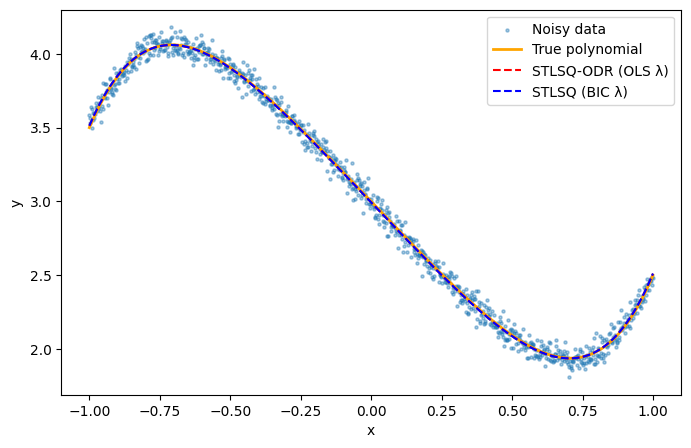
\includegraphics[width=\linewidth]{MSc_Statistics_Research_Report_Template/images/2 0.05.png}
    \subcaption{$\sigma = 0.05$}
\end{minipage}
\begin{minipage}{0.45\textwidth}
    \centering
    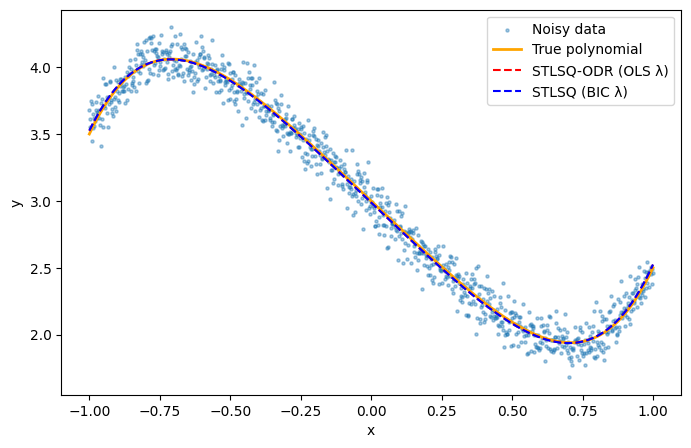
\includegraphics[width=\linewidth]{MSc_Statistics_Research_Report_Template/images/2 0.1.png}
    \subcaption{$\sigma = 0.1$}
\end{minipage}
\begin{minipage}{0.45\textwidth}
    \centering
    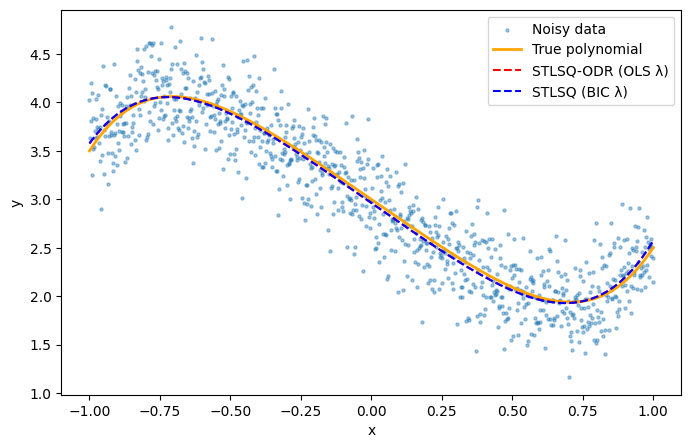
\includegraphics[width=\linewidth]{MSc_Statistics_Research_Report_Template/images/2 0.3.png} 
    \subcaption{$\sigma = 0.3$}
\end{minipage}
\begin{minipage}{0.45\textwidth}
    \centering
    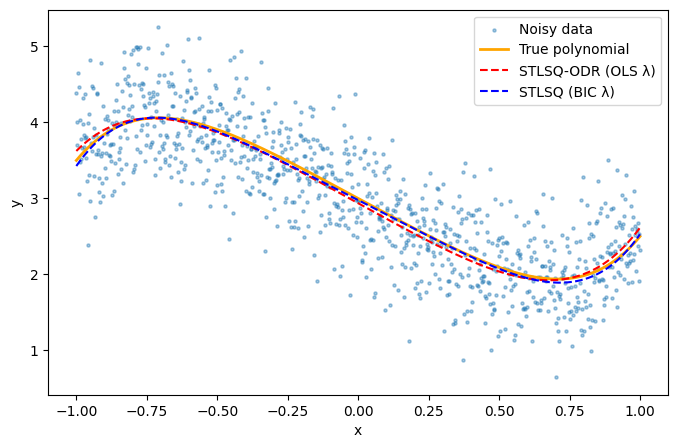
\includegraphics[width=\linewidth]{MSc_Statistics_Research_Report_Template/images/2 0.5.png}
    \subcaption{$\sigma = 0.05$}
\end{minipage}
\caption{Comparison of STLSQ sparse regression results under different Gaussian noise variances $\sigma$.}
\label{fig:stlsq}
\end{figure}

\begin{itemize}
\item Case 1: We add independent Gaussian noise to both input and output variables.

\item Case 2: We add independent Student-t noise to both input and output variables.

\item Case 3: We add correlated Gaussian noise to both input and output variables.

\item Case 4: We add correlated Student-t noise to both input and output variables.
\end{itemize}
we sample $n=1000$ input points uniformly over the domain $[−1,1]$.

We also compare BIC-base and OLS-base to choose different thresholds $\lambda$ in STLSQ\_ODR model selection.
With additive adjustments $\boldsymbol{\delta}_i\in\mathbb{R}^m$ to the predictors and a weighting ratio $d = \sigma_y^{2}/\sigma_x^{2}$,
ODR fits $(w,\{\boldsymbol{\delta}_i\})$ by minimizing
\[
J(\boldsymbol{w},\{\boldsymbol{\delta}_i\}) \;=\; \sum_{i=1}^{n}
\Bigl( y_i - \mathbf{\Phi}(\boldsymbol{x}_i+\boldsymbol{\delta}_i)^\top \boldsymbol{w} \Bigr)^2
\;+\; d\,\|\boldsymbol{\delta}_i\|^2 .
\]



Let $(\widehat{w},\{\widehat{\delta}_i\})$ be the minimizer. We then define the
profiled orthogonal residual sum as
\[
\mathrm{RSS}_{\text{ODR}}
= \sum_{i=1}^{n}
\Bigl( y_i - \mathbf{\Phi}(\boldsymbol{x}_i+\widehat{\boldsymbol{\delta}}_i)^\top \widehat{\boldsymbol{w}} \Bigr)^2
\;+\; d\,\|\widehat{\boldsymbol{\delta}}_i\|^2 ,
\]
and compute
\[
\mathrm{BIC}_{\text{ODR}}
= n\ln\!\Bigl(\tfrac{\mathrm{RSS}_{\text{ODR}}}{n}\Bigr) + k\ln n.
\]
Here $k$ counts the nonzero coefficients in $\widehat{\boldsymbol{w}}$. This replaces the vertical RSS with the profiled orthogonal distance appropriate for EIV.




\paragraph{Case 1}

\begin{table}
\centering
\caption{Comparison of STLSQ-ODR sparse regression results under different Gaussian noise variances $(\sigma_x^2, \sigma_y^2)$.}
\label{tab:sparse_noise}
\scriptsize
\begin{tabular}{c p{6cm} p{6cm}}
\toprule
$(\sigma_x^2, \sigma_y^2)$ & Method 1 (BIC) & Method 2 (OLS$\times 0.9$) \\
\midrule
(0.01, 0.01) & $\lambda=0.0082$\newline coeffs = (3.00, -2.00, 0, 0.50, 0, 1.00) 
             & $\lambda=0.0143$\newline coeffs = (3.00, -2.00 0, 0.50, 0, 1.00) \\
\midrule
(0.05, 0.05) & $\lambda=0.0335$\newline coeffs = (2.99, -2.002, 0, 0.50, 0, 0.96) 
             & $\lambda=0.0272$\newline coeffs = (2.98, -2.00, 0.07, 0.54, -0.07, 0.92) \\
\midrule
(0.1, 0.1)   & $\lambda=0.0677$\newline coeffs = (2.996, -2.00, 0, 0.53, 0, 0.86) 
             & $\lambda=0.0195$\newline coeffs = (2.97, -2.03, 0.12, 0.72, -0.13, 0.67) \\
\midrule
(0.2, 0.2)   & $\lambda=0.0602$\newline coeffs = (2.98, -2.42, 0, 2.21, 0, -0.61) 
             & $\lambda=0.0121$\newline coeffs = (2.95, -2.32, 0.13, 2.06, -0.08, -0.58) \\
\midrule
(0.3, 0.3)   & $\lambda=0.0335$\newline coeffs = (2.98, -2.52, 0, 2.13, 0, -0.50) 
             & $\lambda=0.0053$\newline coeffs = (2.96, -2.59, 0.06, 2.58, 0, -0.77) \\
\midrule
(0.4, 0.4)   & $\lambda=0.4954$\newline coeffs = (2.99, -1.12, 0, 0, 0, 0) 
             & $\lambda=0.0242$\newline coeffs = (2.99, -3.00, 0, 2.90, 0, -0.71) \\
\bottomrule
\end{tabular}
\end{table}

\begin{figure}
\centering
\begin{minipage}{0.45\textwidth}
    \centering
    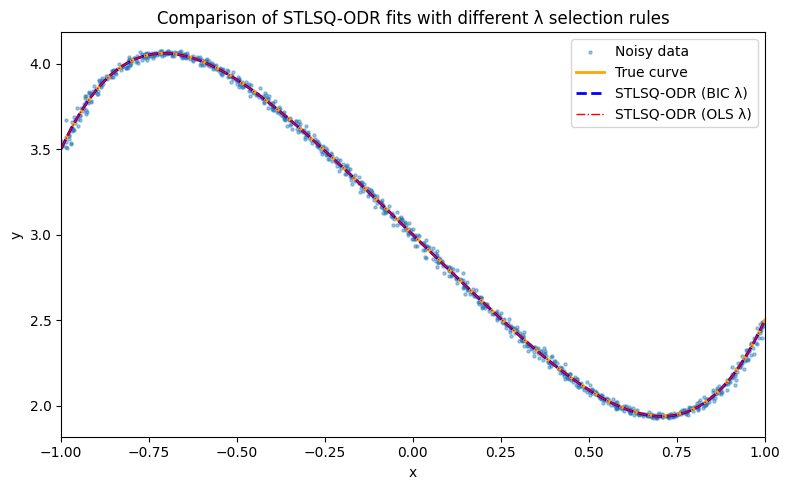
\includegraphics[width=\linewidth]{MSc_Statistics_Research_Report_Template/images/0.01,0.01.png}
    \subcaption{$\sigma_x^2 = 0.01, \; \sigma_y^2 = 0.01$}
\end{minipage}
\begin{minipage}{0.45\textwidth}
    \centering
    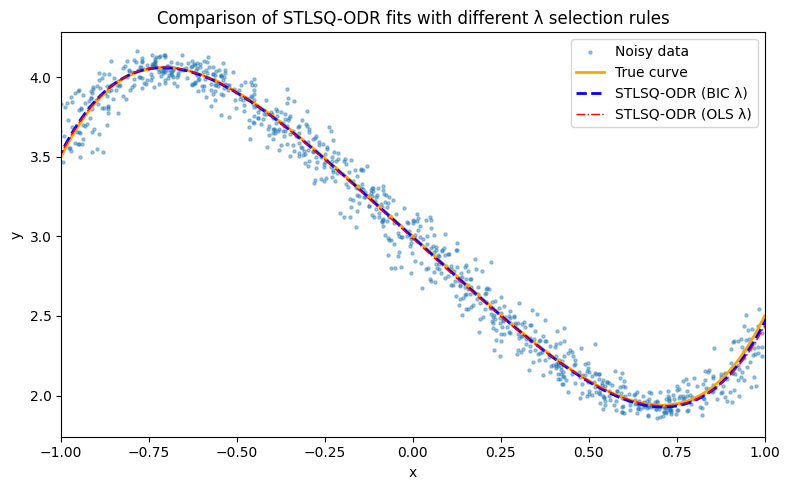
\includegraphics[width=\linewidth]{MSc_Statistics_Research_Report_Template/images/0.05, 0.05.png}
    \subcaption{$\sigma_x^2 = 0.05, \; \sigma_y^2 = 0.05$}
\end{minipage}

\begin{minipage}{0.45\textwidth}
    \centering
    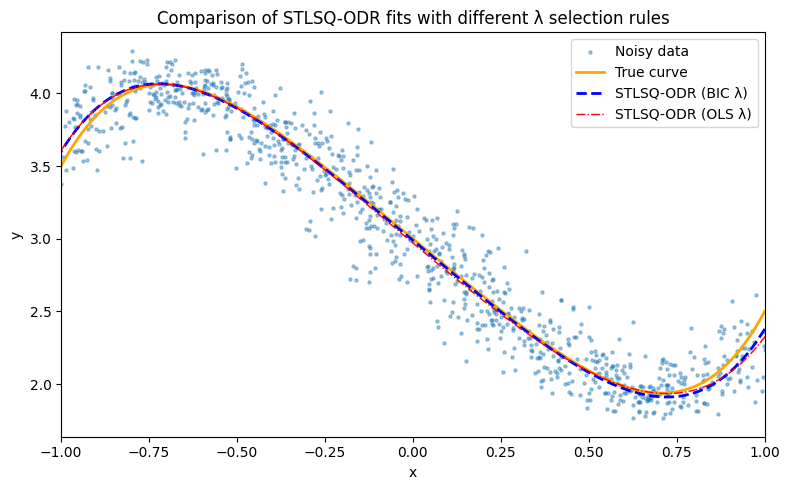
\includegraphics[width=\linewidth]{MSc_Statistics_Research_Report_Template/images/0.1, 0.1.png}
    \subcaption{$\sigma_x^2 = 0.1, \; \sigma_y^2 = 0.1$}
\end{minipage}
\begin{minipage}{0.45\textwidth}
    \centering
    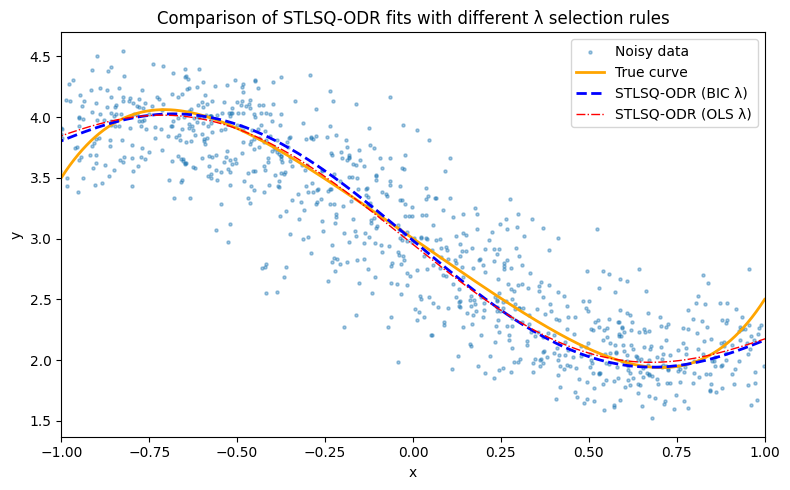
\includegraphics[width=\linewidth]{MSc_Statistics_Research_Report_Template/images/0.2, 0.2.png}
    \subcaption{$\sigma_x^2 = 0.2, \; \sigma_y^2 = 0.2$}
\end{minipage}

\begin{minipage}{0.45\textwidth}
    \centering
    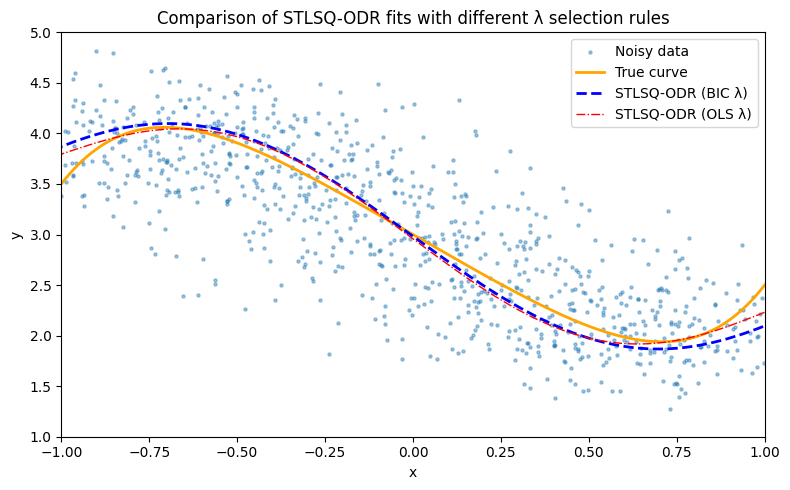
\includegraphics[width=\linewidth]{MSc_Statistics_Research_Report_Template/images/0.3,0.3.png}
    \subcaption{$\sigma_x^2 = 0.3, \; \sigma_y^2 = 0.3$}
\end{minipage}
\begin{minipage}{0.45\textwidth}
    \centering
    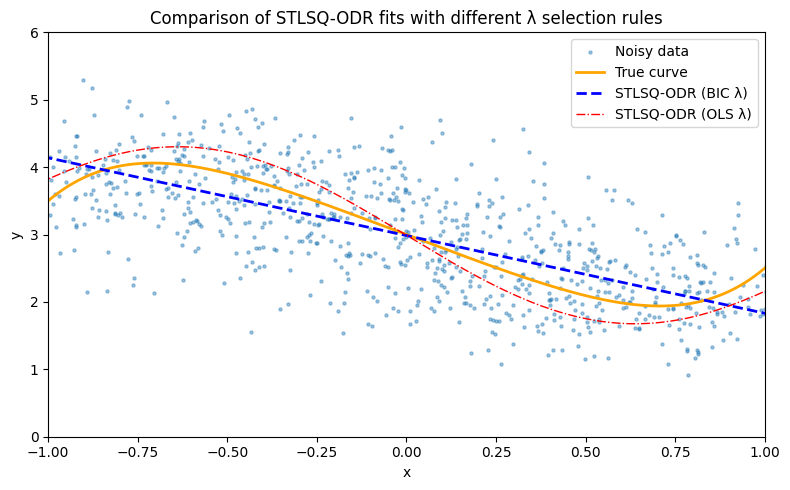
\includegraphics[width=\linewidth]{MSc_Statistics_Research_Report_Template/images/0.4,0.4.png}
    \subcaption{$\sigma_x^2 = 0.4, \; \sigma_y^2 = 0.4$}
\end{minipage}
\caption{Comparison of STLSQ-ODR sparse regression results under different Gaussian noise variances $(\sigma_x^2, \sigma_y^2)$}
\label{fig:stlsq_odr_g}
\end{figure}


Table \ref{tab:sparse_noise} and Figure \ref{fig:stlsq_odr_g} illustrate the performance of STLSQ-ODR under varying Gaussian noise variances $(\sigma_x^2,\sigma_y^2)$. When the noise is small ($\sigma_x^2=\sigma_y^2=0.01$), both BIC-based and OLS-based $\lambda$ selection rules successfully recover the correct sparse polynomial structure. However, once the noise variance exceeds approximately $0.05$, the OLS-based rule fails to shrink irrelevant coefficients to zero, while the BIC-based method continues to make correct model selections as long as the noise remains moderate.



When the noise becomes large ($\sigma^2 \geq 4$), both methods fail to identify the true model structure and produce biased coefficient estimates, indicating the breakdown of sparse recovery under high noise. In particular, the BIC-based method tends to oversimplify the model by shrinking towards an incorrect linear form.



\paragraph{Case 2}

Under Student-$t$ noise, the performance of STLSQ-ODR demonstrates similar patterns as in the Gaussian case, but with more pronounced instability due to heavy-tailed perturbations. As shown in Table \ref{tab:sparse_noise2} and Figure \ref{fig:stlsq_odr_t}, when the noise variance is small ($\sigma^2 \leq 0.01$), both the BIC-based and OLS-based $\lambda$ selection methods successfully recover the true polynomial structure with accurate coefficient estimates. However, once the noise level increases to $\sigma^2 \geq 0.05$, the OLS-based method already fails to shrink irrelevant coefficients to zero, while the BIC-based method remains relatively robust and continues to produce correct model selection. 

\begin{table}[htbp]
\centering
\caption{Comparison of STLSQ-ODR sparse regression results under different Student-t noise variances $(\sigma_x^2, \sigma_y^2)$.}
\label{tab:sparse_noise2}
\scriptsize
\begin{tabular}{c p{6cm} p{6cm}}
\toprule
$(\sigma_x^2, \sigma_y^2)$ & Method 1 (BIC) & Method 2 (OLS$\times 0.9$) \\
\midrule
(0.01, 0.01) & $\lambda=0.0029$\newline coeffs = (3.00, -2.00, 0, 0.53, 0, 0.97) 
             & $\lambda=0.0047$\newline coeffs = (3.00, -2.00, 0, 0.53, 0, 0.96) \\
\midrule
(0.05, 0.05) & $\lambda=0.3486$\newline coeffs = (3.01, -2.23, 0, 1.55, 0, 0) 
             & $\lambda=0.0280$\newline coeffs = (3.01, -2.05, 0, 0.82, 0, 0.62) \\
\midrule
(0.1, 0.1)   & $\lambda=0.1081$\newline coeffs = (3.01, -2.38, 0, 2.00, 0, -0.38) 
             & $\lambda=0.0754$\newline coeffs = (3.03, -2.36, -0.20, 2.11, 0.21, -0.52) \\
\midrule
(0.2, 0.2)   & $\lambda=0.4406$\newline coeffs = (3.03, -1.14, 0, 0, 0, 0) 
             & $\lambda=0.0206$\newline coeffs = (3.08, -2.08, -0.31, 1.22, 0.17, -0.14) \\
\bottomrule
\end{tabular}
\end{table}

When the noise becomes moderate ($\sigma^2 = 0.1$ or $0.2$), both methods exhibit degraded performance, with the BIC-based method tending to oversimplify the model by collapsing to an incorrect linear form, whereas the OLS-based method produces biased estimates with spurious nonzero terms. This highlights the additional difficulty of sparse recovery under heavy-tailed noise, where extreme perturbations significantly affect stability and reliability of coefficient estimation.

\begin{figure}[htbp]
\centering
\begin{minipage}{0.45\textwidth}
    \centering
    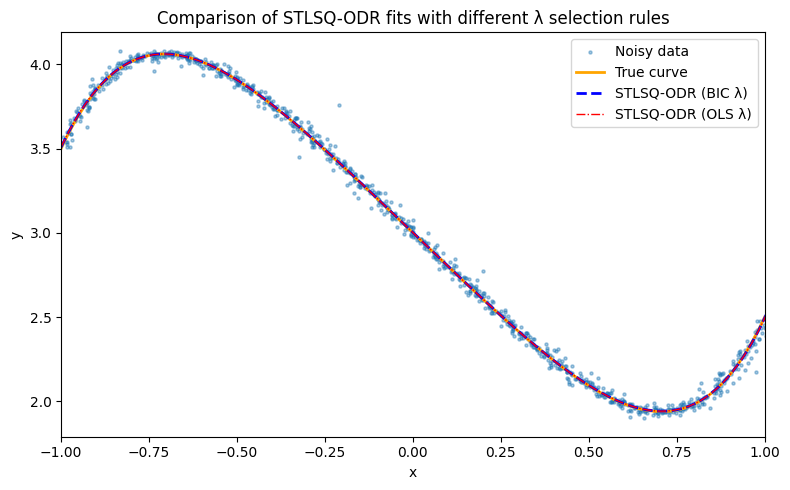
\includegraphics[width=\linewidth]{MSc_Statistics_Research_Report_Template/images/t10.01,0.01.png}
    \subcaption{$\sigma_x^2 = 0.01, \; \sigma_y^2 = 0.01$}
\end{minipage}
\begin{minipage}{0.45\textwidth}
    \centering
    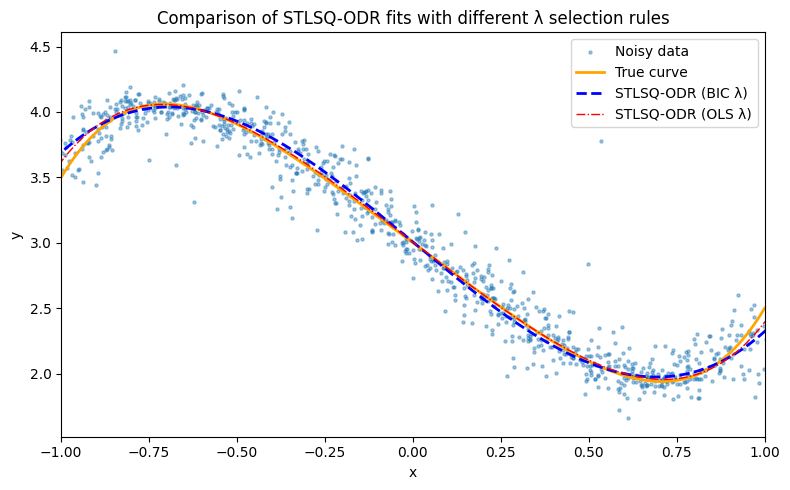
\includegraphics[width=\linewidth]{MSc_Statistics_Research_Report_Template/images/t 0.05,0.05.png}
    \subcaption{$\sigma_x^2 = 0.05, \; \sigma_y^2 = 0.05$}
\end{minipage}

\begin{minipage}{0.45\textwidth}
    \centering
    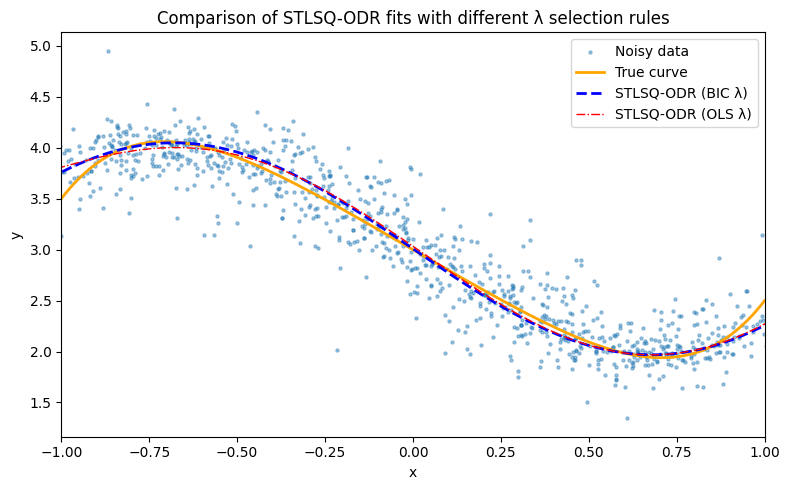
\includegraphics[width=\linewidth]{MSc_Statistics_Research_Report_Template/images/t0.1,0.1.png} 
    \subcaption{$\sigma_x^2 = 0.1, \; \sigma_y^2 = 0.1$}
\end{minipage}
\begin{minipage}{0.45\textwidth}
    \centering
    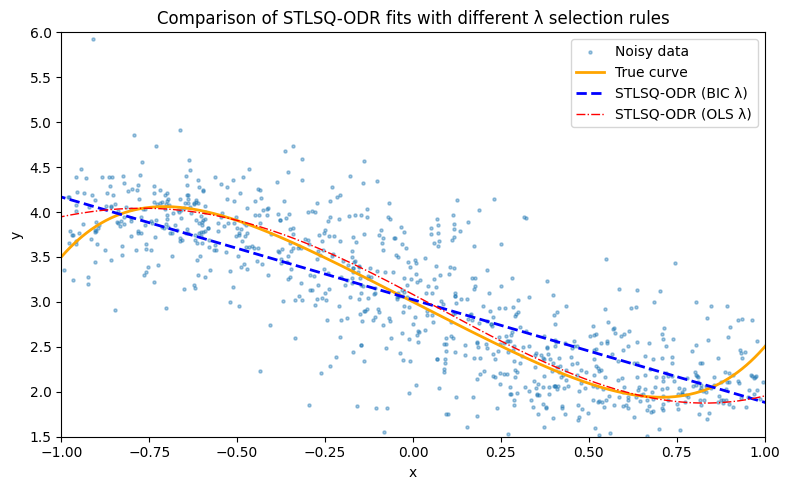
\includegraphics[width=\linewidth]{MSc_Statistics_Research_Report_Template/images/t0.2,0.2.png}
    \subcaption{$\sigma_x^2 = 0.2, \; \sigma_y^2 = 0.2$}
\end{minipage}

\caption{Comparison of STLSQ-ODR sparse regression results under different Student-t noise variances $(\sigma_x^2, \sigma_y^2)$.}
\label{fig:stlsq_odr_t}
\end{figure}

\paragraph{Case 3}

To further examine the effect of correlated Gaussian noise, we consider the case where both predictor and response variables are perturbed with correlated Gaussian errors of equal variance $\sigma_x^2 = \sigma_y^2$, under varying correlation levels $\rho \in [0.1, 1.0]$. As shown in Table \ref{tab:cor}, the sparse recovery results demonstrate that the BIC-based thresholding method generally outperforms the OLS-based method. In particular, for low to moderate noise levels ($\sigma_x = \sigma_y \leq 0.05$), the BIC-based method consistently recovers the correct polynomial structure with accurate coefficient estimates, whereas the OLS-based method tends to include additional small spurious terms, reflecting reduced stability under correlated noise.
As the noise variance increases, this performance gap becomes more evident. For example, at $\sigma_x = \sigma_y = 0.05$ with $\rho=1.0$, the OLS-based method admits extra nonzero terms, while the BIC-based method still maintains sparsity and accurate recovery. This highlights the stronger robustness of the BIC-based criterion in balancing model fit and complexity under correlated perturbations.

However, when the noise level becomes large ($\sigma_x = \sigma_y = 0.07, \rho=1.0$), even the BIC-based method fails to correctly identify the true model. This breakdown indicates that under high-variance correlated Gaussian noise, the signal-to-noise ratio becomes too low for reliable sparse recovery.

\begin{table}[htbp]
\centering
\caption{Comparison of sparse regression results under different correlation levels $\rho$ and Gaussian noise scales $\sigma_x$, $\sigma_y$.}
\label{tab:cor}
\scriptsize
\begin{tabular}{c c p{6cm} p{6cm}}
\toprule
$\sigma_x,\sigma_y$ & $\rho$ & Method 1 (BIC) & Method 2 (OLS$\times 0.9$) \\
\midrule
0.01 & 0.1 
& $\lambda=0.0058$\newline coeffs = (3.00, -2.01, 0, 0.53, 0, 0.97) 
& $\lambda=0.0041$\newline coeffs = (3.00, -2.01, 0.01, 0.53, -0.01, 0.97) \\
\midrule
0.01 & 1.0 
& $\lambda=0.0092$\newline coeffs = (3.00, -2.01, 0, 0.52, 0, 0.98) 
& $\lambda=0.0065$\newline coeffs = (3.00, -2.01, 0.02, 0.52, -0.02, 0.98) \\
\midrule
0.05 & 0.1 
& $\lambda=0.0236$\newline coeffs = (3.00, -2.03, 0, 0.57, 0, 0.93) 
& $\lambda=0.0226$\newline coeffs = (3.00, -2.03, 0.04, 0.56, -0.05, 0.94) \\
\midrule
0.05 & 1.0 
& $\lambda=0.0298$\newline coeffs = (3.00, -2.07, 0, 0.68, 0, 0.88) 
& $\lambda=0.0232$\newline coeffs = (2.99, -2.07, 0.06, 0.68, -0.06, 0.89) \\
\midrule
0.07 & 1.0 
& $\lambda=0.3919$\newline coeffs = (3.00, -2.34, 0, 1.71, 0, 0) 
& $\lambda=0.0362$\newline coeffs = (2.99, -2.12, 0.08, 0.77, -0.09, 0.86) \\
\bottomrule
\end{tabular}
\end{table}




\paragraph{Case 4}

We consider the case where both input and output variables are perturbed with correlated Student-t noise of equal variance $\sigma_x^2 = \sigma_y^2 = 0.02$. As shown in Table \ref{tab:sparse_rho}, the sparse recovery results remain relatively stable across different correlation levels $\rho \in [0.1, 1.0]$. Both BIC-based and OLS-based $\lambda$ selection methods consistently identify the correct polynomial structure, with coefficient estimates close to the ground truth. 

However, a gradual increase in correlation slightly reduces the sparsity and stability of the OLS-based method, leading to the inclusion of small spurious terms when $\rho=1.0$. In contrast, the BIC-based method remains more conservative, maintaining exact sparsity throughout all correlation levels. These findings suggest that while correlated noise does not fundamentally impair sparse recovery at moderate noise levels, it can introduce additional estimation bias in OLS-based selection, whereas BIC-based selection exhibits stronger robustness.

\begin{table}[htbp]
\centering
\caption{Comparison of sparse regression results under different correlation levels $\rho$ when Student-t noise scales are $\sigma_x=0.02$ and $\sigma_y=0.02$. }
\label{tab:sparse_rho}
\scriptsize
\begin{tabular}{c p{6cm} p{6cm}}
\toprule
$\rho$ & Method 1 (BIC) & Method 2 (OLS$\times 0.9$) \\
\midrule
0.1 & $\lambda=0.0018$\newline coeffs = (3.00, -2.04, 0, 0.68, 0, 0.81) 
    & $\lambda=0.0542$\newline coeffs = (3.00, -2.03, 0, 0.62, 0, 0.88) \\
\midrule
0.5 & $\lambda=0.0013$\newline coeffs = (3.00, -2.06, 0, 0.73, 0, 0.78) 
    & $\lambda=0.0371$\newline coeffs = (3.00, -2.04, 0, 0.65, 0, 0.87) \\
\midrule
0.8 & $\lambda=0.0032$\newline coeffs = (3.00, -2.06, 0, 0.75, 0, 0.77) 
    & $\lambda=0.0313$\newline coeffs = (3.00, -2.051, 0, 0.65, 0, 0.88) \\
\midrule
1.0 & $\lambda=0.0131$\newline coeffs = (3.00, -2.06, 0, 0.74, 0, 0.80) 
    & $\lambda=0.0262$\newline coeffs = (3.00, -2.04, 0.05, 0.59, -0.06, 0.94) \\
\bottomrule
\end{tabular}
\end{table}




















\section{Conclusion and Discussion}
\label{sec:disc}

This study introduces two complementary frameworks for sparse polynomial model selection in noisy settings:
The first uses Bayesian evidence when only the response is noisy and an ODR approach for the EIV setting, where noise affects both the predictors and the response.
The main findings can be summarised as follows:
\begin{itemize}
    \item The Bayesian razor method reliably identifies parsimonious models under moderate response noise, directly quantifying posterior model probabilities in accordance with Occam’s razor.
    
    The simulation experiments for the Bayesian razor method demonstrated that, in the case where noise is added only to the response variable, the method consistently identified the correct polynomial structure under low to moderate noise levels. Posterior probabilities were strongly concentrated on the true model, and coefficient estimates closely matched the ground truth. Although the noise variance increased, the Bayesian razor still maintained accurate model selection up to relatively high noise levels. Only when the noise variance became excessively large (e.g., $\sigma \ge 3.9$) did the method break down. These findings highlight the robustness of Bayesian evidence in balancing model fit and complexity in the presence of response noise.
    \item The STLSQ framework provides a simple and efficient approach for enforcing sparsity in polynomial regression, but its performance degrades under increasing response noise. But both methods failed to select the exact sparse solution.

    In the simulations, both the OLS-based and BIC-based thresholding rules produced coefficient estimates close to the ground truth. However, as the noise variance increased ($\sigma = 0.3, 0.5$), the recovered coefficients became increasingly biased. Although the BIC-based strategy generally yielded more stable fits than the OLS-based rule, neither approach was able to maintain correct sparsity. 

    \item The STLSQ-ODR framework effectively mitigates bias caused by noisy predictors, showing robust recovery of governing equations under Gaussian, Student-t, and correlated noise.
    
    In the EIV problem where both predictors and responses were contaminated with Gaussian, Student-t, and correlated noise, the proposed STLSQ-ODR framework exhibited strong recovery of the true sparse polynomial structure under small to moderate noise. Both OLS-based and BIC-based thresholding strategies worked well in the low-noise regime, but as the noise increased, the BIC-based approach consistently outperformed the OLS-based rule by eliminating spurious terms and preserving sparsity. Under heavy-tailed and correlated noise, BIC-based selection remained relatively stable, while OLS-based methods became less reliable and tended to include irrelevant coefficients. Although both approaches eventually failed when the noise level was too large, the overall results confirm that STLSQ-ODR provides a robust and noise-aware mechanism for sparse recovery in challenging settings.
    \item across noise regimes, BIC-based thresholding demonstrates stronger stability than OLS-based selection, though both methods deteriorate when noise becomes excessively large.
\end{itemize}

During the simulation studies, we identified limitations inherent in the model selection approaches used. For the Bayesian razor method, reliable performance hinges on the assumption that only response noise is present. Once predictor variables are corrupted, the likelihood structure becomes intractable, rendering direct Bayesian evidence calculations infeasible. Approximate Bayesian methods, such as variational inference or MCMC with latent predictor modelling \citep{gunapati2022}, could be explored as future work. For the STLSQ-ODR framework, the simulation results revealed sensitivity to the choice of threshold $\lambda$: while BIC-based selection proved relatively robust, it tended to oversimplify models under heavy-tailed or high-variance noise, collapsing sparse polynomials into incorrect linear approximations. Moreover, both approaches rely on synthetic datasets with controlled noise structures, which may not fully reflect the heterogeneity and dependence encountered in real experimental measurements. Finally, the one-dimensional polynomial setting considered here represents a simplified testbed; scaling these methods to multivariate and high-dimensional systems remains an open challenge, where identifiability and computational tractability may be severely strained.

Overall, the main findings appear robust under moderate noise but degrade when the signal-to-noise ratio falls below a critical threshold. In such regimes, both Bayesian evidence and ODR-based methods exhibit systematic biases—underscoring that no estimator is immune to extreme noise contamination. Nevertheless, the complementarity of the two approaches is that Bayesian razor excels in balancing fit and complexity when predictor variables are reliable, while STLSQ-ODR provides resilience when both predictors and responses are noisy. This suggests a promising future direction in combining Bayesian evidence with ODR-based sparsification into a unified framework, enabling comprehensive and principled model selection across a broad range of noisy scenarios.
\section{Endmatter} 
\label{sec:endmatter}

All the code used for this project can be found at: \url{https://github.com/Xinyi10086/project/releases/tag/Project}.
All the results can be reproduced by the code.








\clearpage

%%References part of the main text
% References: modify the file refs.bib
\bibliographystyle{apalike}
\bibliography{refs}

\clearpage

%=========================================================
%% Create supplementary material 
%
%
% - Providing supplementary materials to your report is voluntary and will not normally be read by your examiners.
% - If you wish to include supplementary materials, add these by modifying the file 
%   `supplementary.tex`
% - otherwise deactive the include command below
%
%
%=========================================================

%% reset page counter and start appendix pages numbering
\pagenumbering{arabic}
\renewcommand*{\thepage}{Supplementary Material Page \arabic{page}}
\renewcommand{\thesection}{\Alph{section}}
%% Supplementary Material goes here
\appendix
\include{supplementary}
%=========================================================


\end{document}
